\documentclass{article}
% \VignettePackage{dapc}
% \VignetteIndexEntry{An introduction to Discriminant Analysis of Principal Components (DAPC)}

\usepackage{graphicx}
\usepackage[colorlinks=true,urlcolor=blue]{hyperref}
\usepackage{array}
\usepackage{color}

\usepackage[utf8]{inputenc} % for UTF-8/single quotes from sQuote()


% for bold symbols in mathmode
\usepackage{bm}

\newcommand{\R}{\mathbb{R}}
\newcommand{\beq}{\begin{equation}}
\newcommand{\eeq}{\end{equation}}
\newcommand{\m}[1]{\mathbf{#1}}



\newcommand{\code}[1]{{{\tt #1}}}
\title{A tutorial for Discriminant Analysis of Principal Components (DAPC) using \textit{adegenet} 1.3-0}
\author{Thibaut Jombart}
\date{\today}




\sloppy
\hyphenpenalty 10000


\usepackage{Sweave}
\begin{document}





\definecolor{Soutput}{rgb}{0,0,0.56}
\definecolor{Sinput}{rgb}{0.56,0,0}
\DefineVerbatimEnvironment{Sinput}{Verbatim}
{formatcom={\color{Sinput}},fontsize=\footnotesize, baselinestretch=0.75}
\DefineVerbatimEnvironment{Soutput}{Verbatim}
{formatcom={\color{Soutput}},fontsize=\footnotesize, baselinestretch=0.75}

\color{black}

\maketitle

\begin{abstract}
  This vignette provides a tutorial for applying the Discriminant Analysis of Principal Components
  (DAPC \cite{tjart19}) using the \textit{adegenet} package \cite{tjart05} for the R software
  \cite{np145}. This methods aims to identify and describe genetic clusters, although it can in fact
  be applied to any quantitative data. We illustrate how to use \code{find.clusters} to identify
  clusters, and \code{dapc} to describe the relationships between these clusters. More advanced
  topics are then introduced, such as advanced graphics, assessing the stability of DAPC results and
  using supplementary individuals.
\end{abstract}


\newpage
\tableofcontents


\newpage
%%%%%%%%%%%%%%%%
%%%%%%%%%%%%%%%%
\section{Introduction}
%%%%%%%%%%%%%%%%
%%%%%%%%%%%%%%%%


Investigating genetic diversity using multivariate approaches relies on finding synthetic variables
built as linear combinations of alleles (i.e. $\mbox{new-variable} = a_1 \mbox{allele}_1 + a_2 \mbox{allele}_2 + ... $
where $a_1$, $a_2$ etc. are real coefficients)
and which reflect as well as possible the genetic variation amongst the studied individuals.
However, most of the time we are not only interested in the diversity amongst individuals, but
also and possibly more so in the diversity between groups of individuals.
Typically, one will be analysing individual data to identify populations, or more largely genetic
clusters, and then describe these clusters.

A problem occuring in traditional methods is they usually focus on the entire genetic variation.
Genetic variability can be decomposed using a standard multivariate ANOVA model as:
$$
\mbox{total variance} = \mbox{(variance between groups)} + \mbox{(variance within groups)}
$$
or more simply, denoting $\m{X}$ the data matrix:
$$
VAR(\m{X}) = B(\m{X}) + W(\m{X})
$$

Usual approaches such as Principal Component Analysis (PCA) or Principal Coordinates
Analysis (PCoA / MDS) focus on $VAR(\m{X})$. That is, they only describe the global diversity,
possibly overlooking differences between groups. On the contrary, DAPC optimizes $B(\m{X})$ while
minimizing $W(\m{X})$: it seeks synthetic variables, the \textit{discriminant functions}, which show
differences between groups as best as possible while minimizing variation within clusters.










%%%%%%%%%%%%%%%%
%%%%%%%%%%%%%%%%
\section{Identifying clusters using \code{find.clusters}}
%%%%%%%%%%%%%%%%
%%%%%%%%%%%%%%%%

%%%%%%%%%%%%%%%%
\subsection{Rationale}
%%%%%%%%%%%%%%%%
DAPC in itself requires prior groups to be defined. However, groups are often unknown or uncertain,
and there is a need for identifying genetic clusters before describing them. This can be achieved
using $k$-means, a clustering algorithm which finds a given number (say, $k$) of groups maximizing the variation between
groups, $B(\m{X})$. To identify the optimal number of clusters, $k$-means is run sequentially with
increasing values of $k$, and different clustering solutions are compared using Bayesian Information
Criterion (BIC). Ideally, the optimal clustering solution should correspond to the lowest BIC. In
practice, the 'best' BIC is often indicated by an elbow in the curve of BIC values as a function of
$k$.
\\


While $k$-means could be performed on the raw data, we prefer running the algorithm after
transforming the data using PCA. This transformation has the major advantage of reducing the
number of variables so as to speed up the clustering algorithm. Note that this does not imply a necessary
loss of information since all the principal components (PCs) can be retained, and therefore all the variation in the original data.
In practice however, a reduced number of PCs is often sufficient to identify the existing clusters,
while making the analysis essentially instantaneous.


%%%%%%%%%%%%%%%%
\subsection{In practice}
%%%%%%%%%%%%%%%%

Identification of the clusters is achieved by \code{find.clusters}. This function first transforms
the data using PCA, asking the user to specify the number of retained PCs interactively unless the
argument \code{n.pca} is provided. Then, it runs $k$-means algorithm (function \code{kmeans} from
the \textit{stats} package) with increasing values of $k$, unless the argument  \code{n.clust} is
provided, and computes associated summary statistics (by default, BIC).
See \code{?find.clusters} for other arguments.

\code{find.clusters} is a generic function with methods for \texttt{data.frame}, objects with
the class \texttt{genind} (usual genetic markers) and \texttt{genlight} (genome-wide SNP data).
Here, we illustrate its use using a toy dataset simulated in \cite{tjart19}, \texttt{dapcIllus}:
\begin{Schunk}
\begin{Sinput}
> library(adegenet)
> data(dapcIllus)
> class(dapcIllus)
\end{Sinput}
\begin{Soutput}
[1] "list"
\end{Soutput}
\begin{Sinput}
> names(dapcIllus)
\end{Sinput}
\begin{Soutput}
[1] "a" "b" "c" "d"
\end{Soutput}
\end{Schunk}

\texttt{dapcIllus} is a list containing four datasets; we shall only use the first one:
\begin{Schunk}
\begin{Sinput}
> x <- dapcIllus$a
> x
\end{Sinput}
\begin{Soutput}
   #####################
   ### Genind object ### 
   #####################
- genotypes of individuals - 

S4 class:  genind
@call: read.fstat(file = file, missing = missing, quiet = quiet)

@tab:  600 x 140 matrix of genotypes

@ind.names: vector of  600 individual names
@loc.names: vector of  30 locus names
@loc.nall: number of alleles per locus
@loc.fac: locus factor for the  140 columns of @tab
@all.names: list of  30 components yielding allele names for each locus
@ploidy:  2
@type:  codom

Optionnal contents: 
@pop:  factor giving the population of each individual
@pop.names:  factor giving the population of each individual

@other: - empty -
\end{Soutput}
\end{Schunk}
\texttt{x} is a dataset of 600 individuals simulated under an island model (6 islands) for 30 microsatellite markers.
We use \code{find.clusters} to identify clusters, although true clusters are, in this case, known
(and accessible using \texttt{pop(x)}).
We specify that we want to evaluate up to $k=40$ groups (\texttt{max.n.clust=40}):
\begin{Schunk}
\begin{Sinput}
> grp <- find.clusters(x, max.n.clust = 40)
\end{Sinput}
\end{Schunk}

\begin{center}
  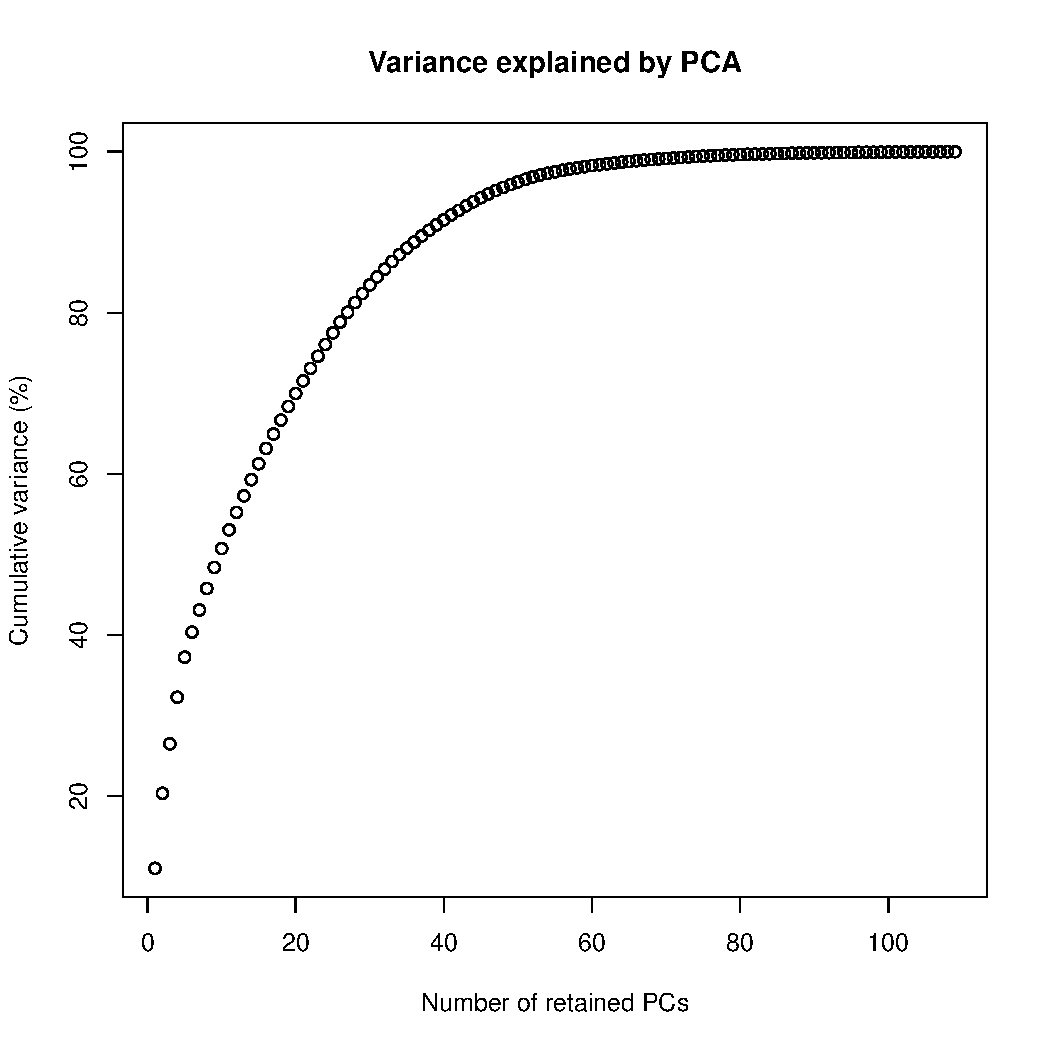
\includegraphics[width=.7\textwidth]{figs/findclust-pca.pdf}
\end{center}

\noindent
The function displays a graph of cumulated variance explained by the eigenvalues of the PCA.
Apart from computational time, there is no reason for keeping a small number of components; here, we
keep all the information, specifying to retain 200 PCs (there are actually less PCs ---around 110---, so all of them
are kept).
\\

Then, the function displays a graph of BIC values for increasing values of $k$:
\begin{center}
  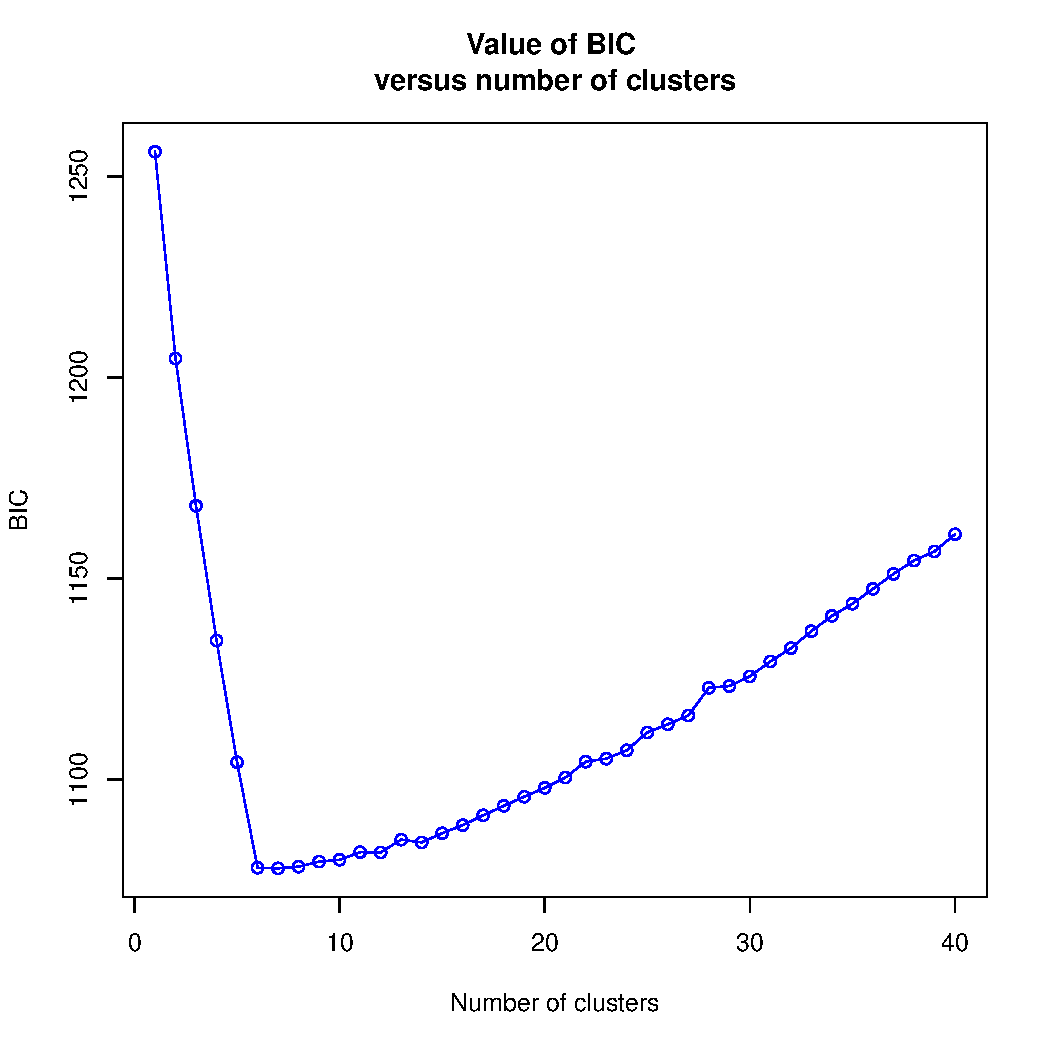
\includegraphics[width=.7\textwidth]{figs/findclust-bic.pdf}
\end{center}

\noindent This graph shows a clear decrease of BIC until $k=6$ clusters, after which BIC increases.
In this case, the elbow in the curve also matches the smallest BIC, and clearly indicates 6 clusters
should be retained. In practice, the choice is often trickier to make for empirical dataset.
\\

The output of \texttt{find.clusters} is a list:
\begin{Schunk}
\begin{Sinput}
> names(grp)
\end{Sinput}
\begin{Soutput}
[1] "Kstat" "stat"  "grp"   "size" 
\end{Soutput}
\begin{Sinput}
> head(grp$Kstat, 8)
\end{Sinput}
\begin{Soutput}
NULL
\end{Soutput}
\begin{Sinput}
> grp$stat
\end{Sinput}
\begin{Soutput}
NULL
\end{Soutput}
\begin{Sinput}
> head(grp$grp, 10)
\end{Sinput}
\begin{Soutput}
001 002 003 004 005 006 007 008 009 010 
  1   1   1   5   1   1   1   1   1   1 
Levels: 1 2 3 4 5 6
\end{Soutput}
\begin{Sinput}
> grp$size
\end{Sinput}
\begin{Soutput}
[1]  98  97 102  99 105  99
\end{Soutput}
\end{Schunk}

The components are respectively the chosen summary statistics (here, BIC) for different values of
$k$ (slot \texttt{Kstat}), the selected number of clusters and the associated BIC (slot
\texttt{stat}), the group memberships (slot \texttt{grp}) and the group sizes (slot \texttt{size}).
Here, since we know the actual groups, we can check how well they have been retrieved by the procedure.
Actual groups are accessed using \texttt{pop}:
\begin{Schunk}
\begin{Sinput}
> table(pop(x), grp$grp)
\end{Sinput}
\begin{Soutput}
      1   2   3   4   5   6
  1  97   0   0   0   3   0
  2   0   0   0  99   1   0
  3   0   2   0   0   0  98
  4   0   0 100   0   0   0
  5   1  95   2   0   2   0
  6   0   0   0   0  99   1
\end{Soutput}
\begin{Sinput}
> table.value(table(pop(x), grp$grp), col.lab = paste("inf", 1:6), 
+     row.lab = paste("ori", 1:6))
\end{Sinput}
\end{Schunk}
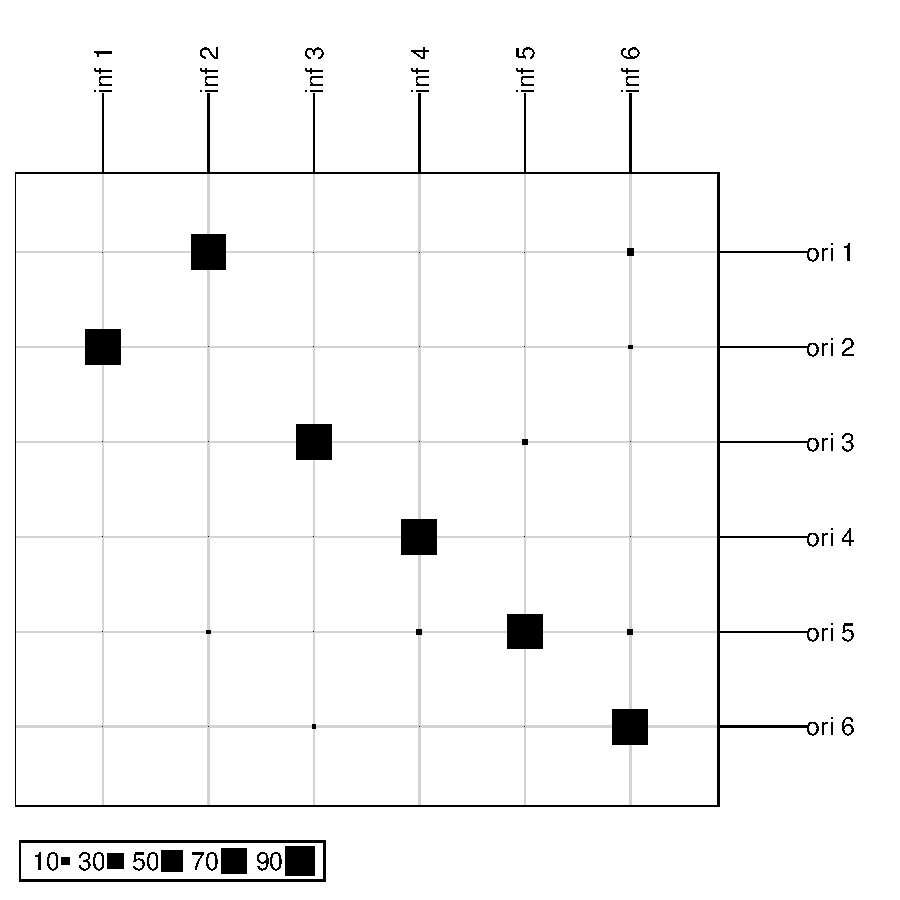
\includegraphics{figs/dapc-006}

\noindent
Rows correspond to actual groups ("ori''), while columns correspond to inferred groups ("inf'').
Here, we can see that original groups have nearly been perfectly identified by the method.


%%%%%%%%%%%%%%%%
\subsection{How many clusters are there really in the data?}
%%%%%%%%%%%%%%%%

Although the most frequently asked when trying to find clusters in genetic data, this question is
equally often meaningless. Clustering algorithms help making a caricature of a complex reality,
which is most of the time far from following known population genetics models. Therefore, we are
rarely looking for actual panmictic populations from which the individuals have been drawn. Genetic
clusters can be biologically meaningful structures and reflect interesting biological processes, but
they are still models.
\\

A slightly different but probably more meaningful question would be: "How many clusters are useful to
describe the data?''. A fundamental point in this question is that clusters are merely tools used to
summarise and understand the data. There is no longer a "true $k$", but some values of $k$ are
better, more efficient summaries of the data than others.
For instance, in the following case:
\begin{center}
  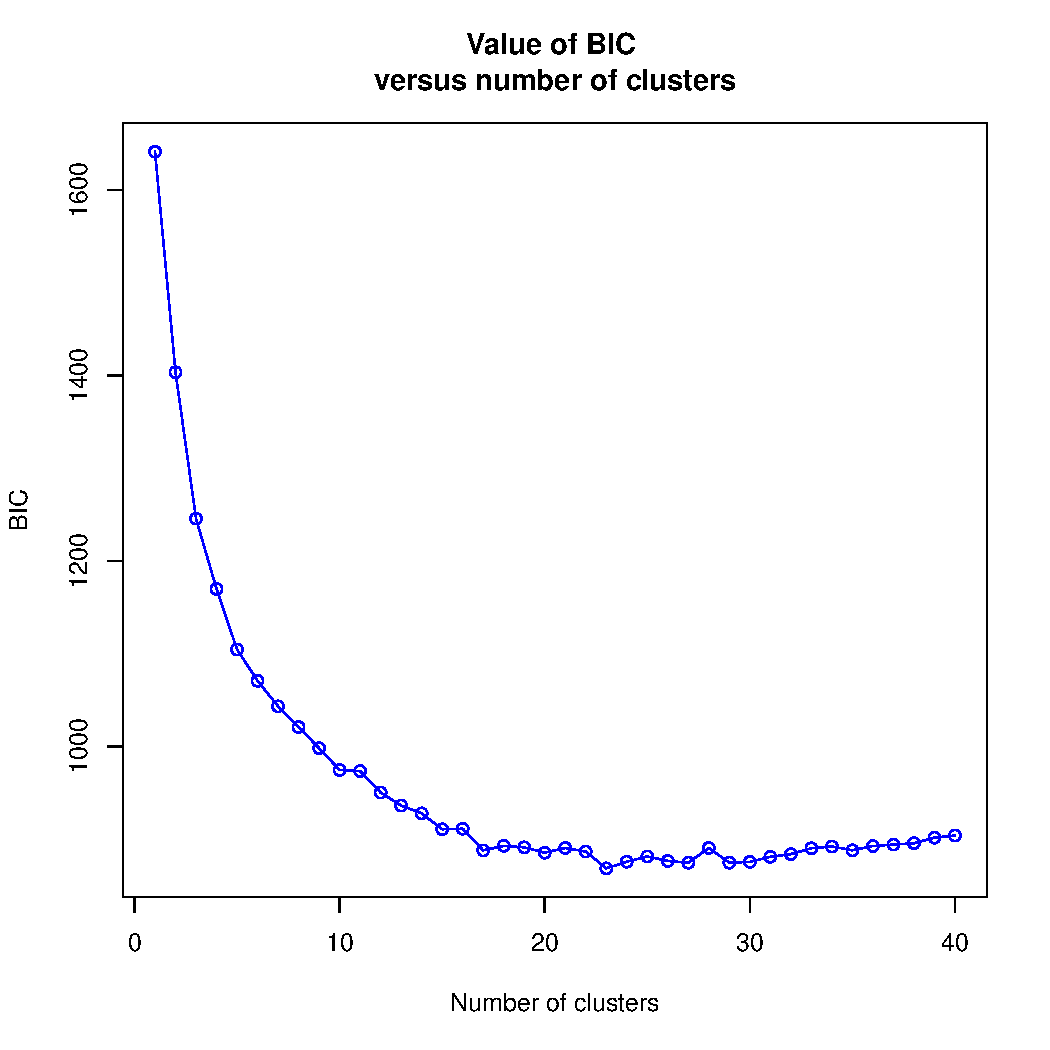
\includegraphics[width=.7\textwidth]{figs/findclust-noclearcut.pdf}
\end{center}

\noindent , the concept of "true $k$" is fairly hypothetical. This does not mean that clutering
algorithms should necessarily be discarded, but surely the reality is more complex than a few
clear-cut, isolated populations. What the BIC decrease says is that 10-20 clusters would provide useful
summaries of the data. The actual number retained is merely a question of personnal taste.









%%%%%%%%%%%%%%%%
%%%%%%%%%%%%%%%%
\section{Describing clusters using \code{dapc}}
%%%%%%%%%%%%%%%%
%%%%%%%%%%%%%%%%


%%%%%%%%%%%%%%%%
\subsection{Rationale}
%%%%%%%%%%%%%%%%
DAPC aims to provide an efficient description of genetic clusters using a few synthetic variables.
These are constructed as linear combinations of the original variables (alleles) which have the
largest between-group variance and the smallest within-group variance. Coefficients of the alleles
used in the linear combination are called \textit{loadings}, while the synthetic variables are
themselves referred to as \textit{discriminant functions}.
\\

Moreover, being based on the Discriminant Analysis, DAPC also provides membership probabilities of
each individual for the different groups based on the retained discriminant functions. While these
are different from the admixture coefficients of software like STRUCTURE, they can still be
interpreted as proximities of individuals to the different clusters. Membership
probabilities also provide indications of how clear-cut genetic clusters are. Loose clusters will
result in fairly flat distributions of membership probabilities of individuals across clusters,
pointing to possible admixture.
\\

Lastly, using the allele loadings, it is possible to represent new individuals (which have not participated to the analysis)
onto the factorial planes, and derive membership probabilities as welll. Such individuals are
referred to as \textit{supplementary individuals}.



%%%%%%%%%%%%%%%%
\subsection{In practice}
%%%%%%%%%%%%%%%%

DAPC is implemented by the function \texttt{dapc}, which first transforms the data using PCA, and
then performs a Discriminant Analysis on the retained principal components. Like
\texttt{find.clusters}, \texttt{dapc} is a generic function with methods for \texttt{data.frame}, and objects with
the class \texttt{genind} (usual genetic markers) and \texttt{genlight} (genome wide SNP data).

We run the analysis on the previous toy dataset, using the inferred groups stored in \texttt{grp\$grp}:

\begin{Schunk}
\begin{Sinput}
> dapc1 <- dapc(x, grp$grp)
\end{Sinput}
\end{Schunk}

The method displays the same graph of cumulated variance as in \texttt{find.cluster}. However, unlike
$k$-means, DAPC can benefit from not using too many PCs. Indeed, retaining too many components with
respect to the number of individuals can lead to over-fitting and unstability in the membership
probabilities returned by the method (see section below about the stability of membership probabilities).

\begin{center}
  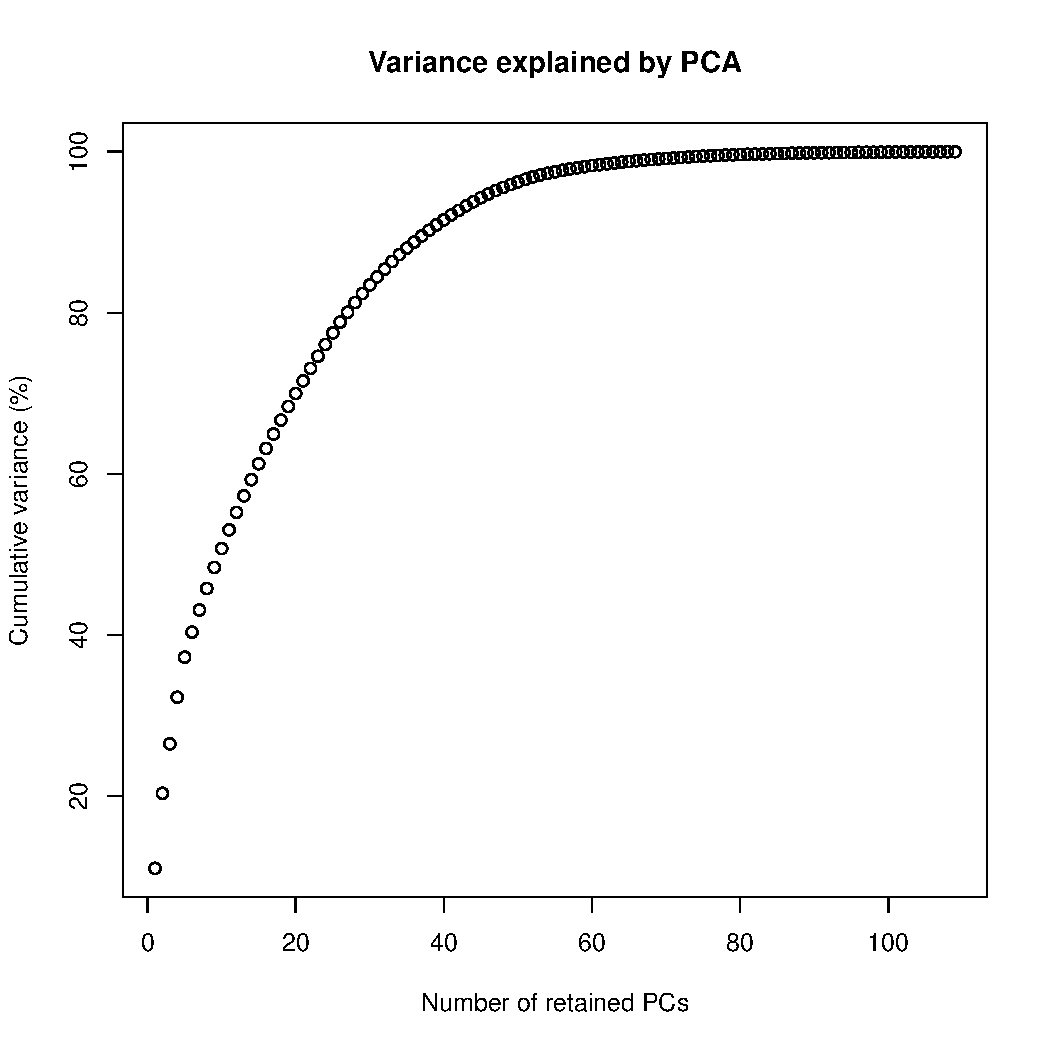
\includegraphics[width=.7\textwidth]{figs/findclust-pca.pdf}
\end{center}

\noindent The bottomline is therefore retaining a few PCs without sacrificing too much information.
Here, we can see that little information is gained by adding PCs after the first 40. We therefore
retain 40 PCs.

Then, the method displays a barplot of eigenvalues for the discriminant analysis, asking for a
number of discriminant functions to retain (unless argument \texttt{n.da} is provided).
\begin{center}
  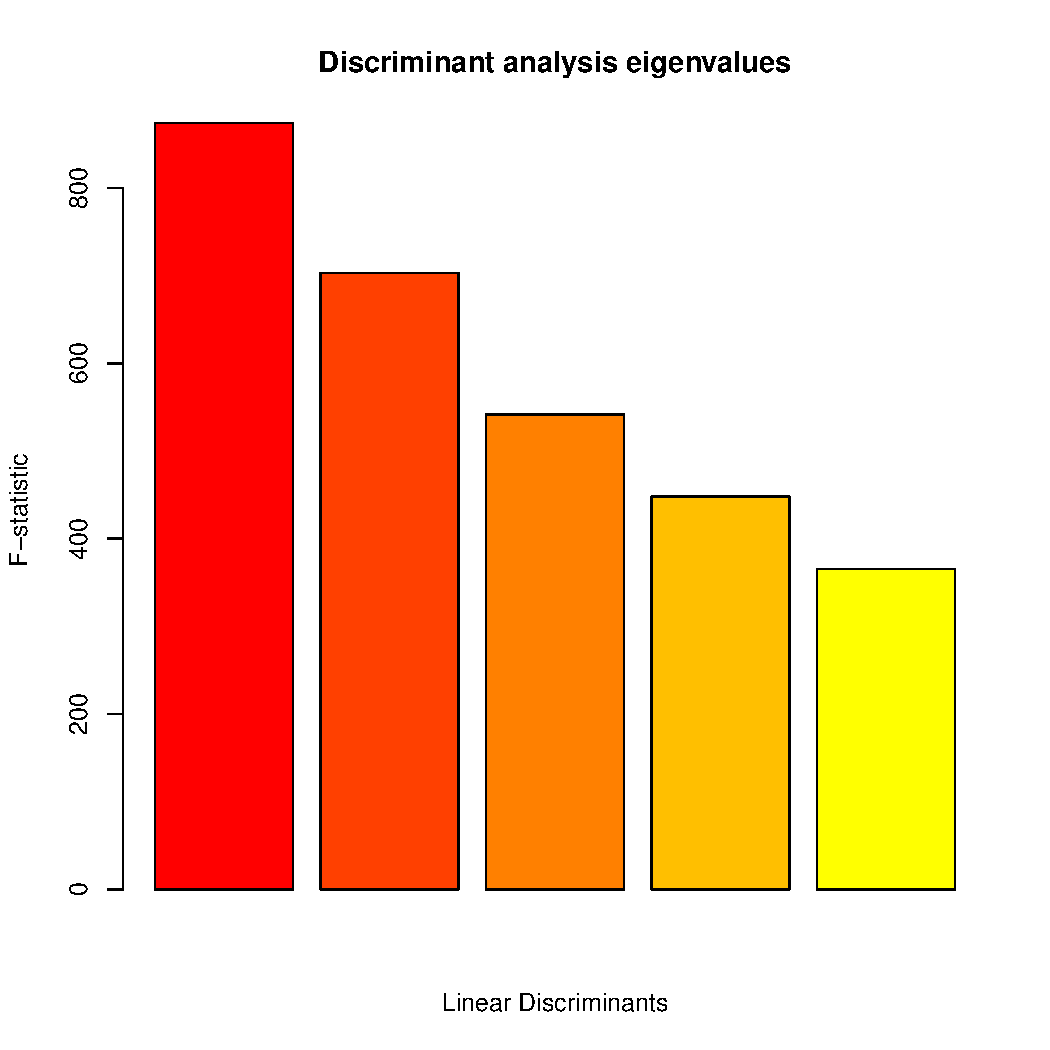
\includegraphics[width=.7\textwidth]{figs/eigen-dapc.pdf}
\end{center}

For small number of clusters, all eigenvalues can be retained since all discriminant functions can
be examined without difficulty. Whenever more (say, tens of) clusters are analysed,
it is likely that the first few dimensions will carry more information than the others, and only
those can then be retained and interpreted.
\\

The object \texttt{dapc1} contains a lot of information:
\begin{Schunk}
\begin{Sinput}
> dapc1
\end{Sinput}
\begin{Soutput}
	#########################################
	# Discriminant Analysis of Principal Components #
	#########################################
class: dapc
$call: dapc.genind(x = x, pop = grp$grp, n.pca = 40, n.da = 100)

$n.pca: 40 first PCs of PCA used
$n.da: 5 discriminant functions saved
$var (proportion of conserved variance): 0.915

$eig (eigenvalues): 874.1 703.2 541.5 447.9 365.3  vector    length content                   
1 $eig      5      eigenvalues               
2 $grp      600    prior group assignment    
3 $prior    6      prior group probabilities 
4 $assign   600    posterior group assignment
5 $pca.cent 140    centring vector of PCA    
6 $pca.norm 140    scaling vector of PCA     
7 $pca.eig  109    eigenvalues of PCA        

  data.frame    nrow ncol content                                          
1 $tab          600  40   retained PCs of PCA                              
2 $means        6    40   group means                                      
3 $loadings     40   5    loadings of variables                            
4 $ind.coord    600  5    coordinates of individuals (principal components)
5 $grp.coord    6    5    coordinates of groups                            
6 $posterior    600  6    posterior membership probabilities               
7 $pca.loadings 140  40   PCA loadings of original variables               
8 $var.contr    140  5    contribution of original variables               
\end{Soutput}
\end{Schunk}

For details about this content, please read the documentation (\texttt{?dapc}).
Essentially, the slots \texttt{ind.coord} and \texttt{grp.coord} contain the coordinates of the
individuals and of the groups used in scatterplots.
Contributions of the alleles to each discriminant function are stored in the slot \texttt{var.contr}.
Eigenvalues, corresponding to the ratio of the variance between groups over the variance within
groups for each discriminant function, are stored in \texttt{eig}.
Basic scatterplots can be obtained using the function \texttt{scatterplot}:
\begin{Schunk}
\begin{Sinput}
> scatter(dapc1)
\end{Sinput}
\end{Schunk}
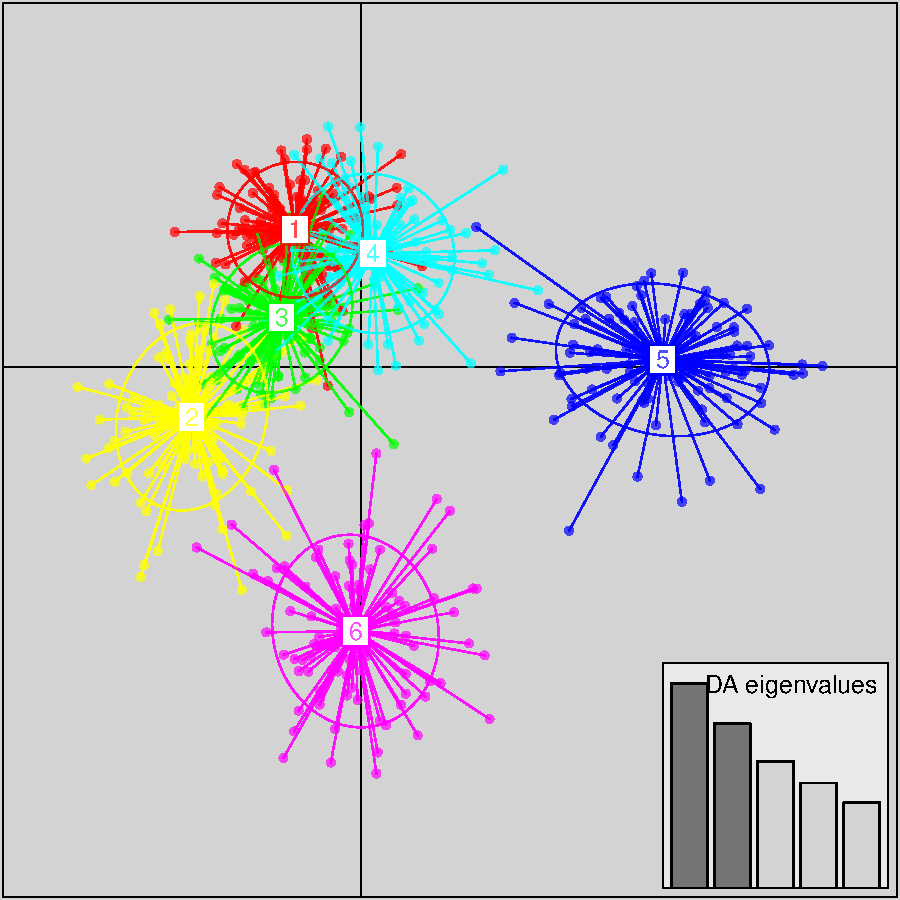
\includegraphics{figs/dapc-010}

\noindent The obtained graph represents the individuals as dots and the groups as inertia
ellipses. Eigenvalues of the analysis are displayed in inset. These graphs are fairly easy to
customize, as shown below.




%%%%%%%%%%%%%%%%
\subsection{Customizing DAPC scatterplots}
%%%%%%%%%%%%%%%%

DAPC scatterplots are the main result of DAPC. It is therefore essential to ensure that information
is displayed efficiently, and if possible to produce pretty figures.
Possibility are almost unlimited, and here we just illustrate a few possibilities offered by
\texttt{scatter}. Note that \texttt{scatter} is a generic function, with a dedicated method for
objects produced by \texttt{dapc}. Documentation of this function can be accessed by typing \texttt{?scatter.dapc}.
\\

We illustrate some graphical possibilities trying to improve the display of the analysis presented
in the previous section.
While the default background (grey) allows to visualize rainbow colors (the default palette for the
groups) more easily, it is not so pretty and is probably better removed for publication purpose.
We also move the inset to a more appropriate place where it does not cover individuals, and use
different symbols for the groups.

\begin{Schunk}
\begin{Sinput}
> scatter(dapc1, posi.da = "bottomright", bg = "white", pch = 17:22)
\end{Sinput}
\end{Schunk}
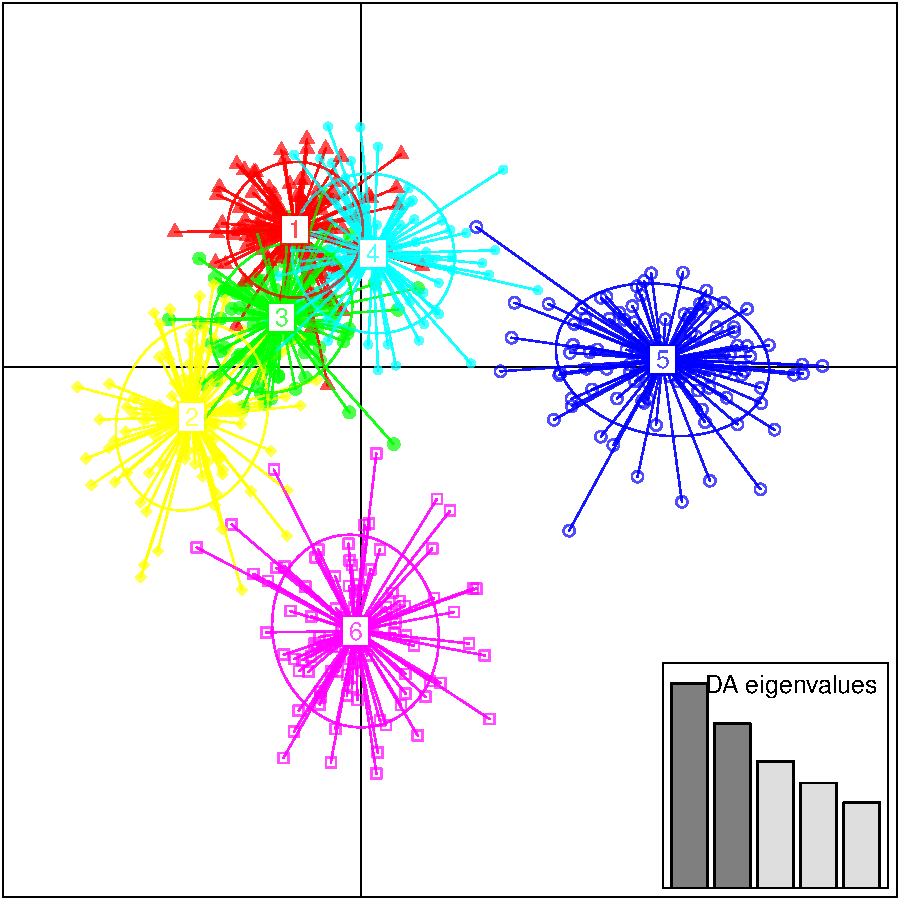
\includegraphics{figs/dapc-011}

\noindent This is still not entirely satisfying: we need to define other colors more visible over a white
background, and we can remove the segments linking the points to their ellipses:
\begin{Schunk}
\begin{Sinput}
> myCol <- c("darkblue", "purple", "green", "orange", "red", "blue")
> scatter(dapc1, posi.da = "bottomright", bg = "white", pch = 17:22, 
+     cstar = 0, col = myCol, scree.pca = TRUE, posi.pca = "bottomleft")
\end{Sinput}
\end{Schunk}
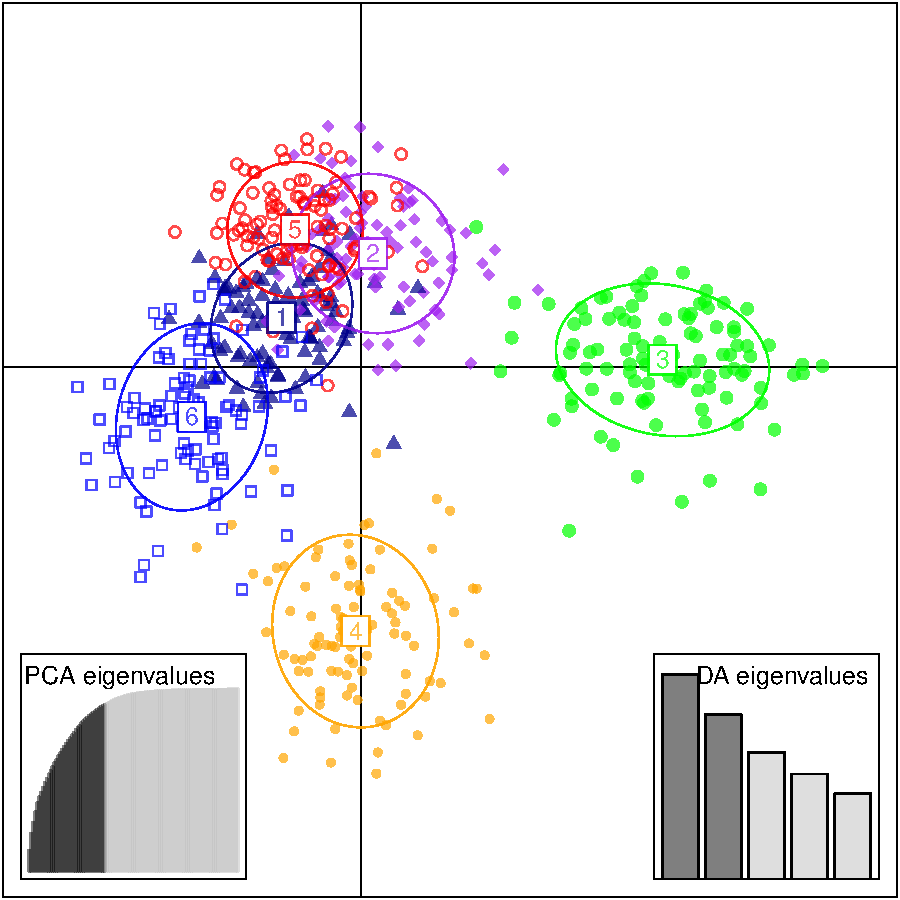
\includegraphics{figs/dapc-012}

\noindent Another possibility is remove the labels within the ellipses and add a legend to the
plot. We also use the same symbol for all individuals, but use bigger dots and transparent colours
to have a better feel for the density of individuals on the factorial plane.
\begin{Schunk}
\begin{Sinput}
> scatter(dapc1, scree.da = FALSE, bg = "white", pch = 20, cell = 0, 
+     cstar = 0, col = myCol, solid = 0.4, cex = 3, clab = 0, leg = TRUE, 
+     txt.leg = paste("Cluster", 1:6))
\end{Sinput}
\end{Schunk}
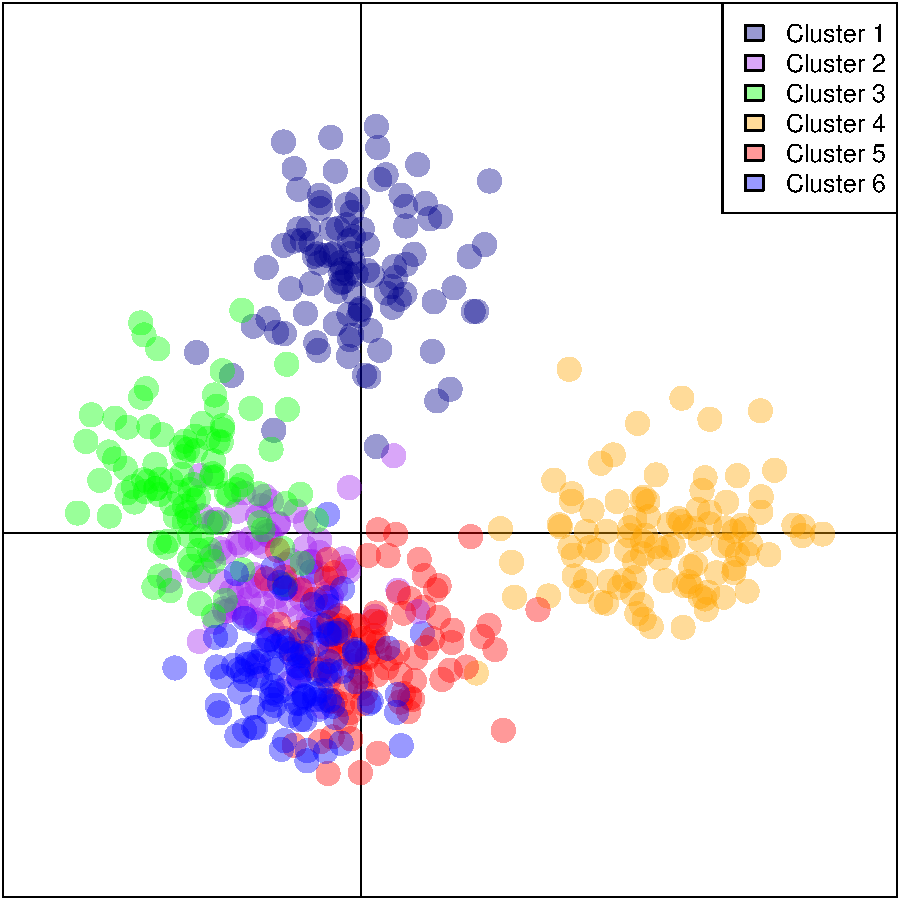
\includegraphics{figs/dapc-013}

We can also add a minimum spanning tree based on the (squared) distances between populations within the
entire space.
This allows one to bear in mind the actual proximities between populations inside the entire space, which are not always
well represented in susbsets of discriminant functions of lesser rank.
We also indicate the centre of each group with crosses.
Lastly, we remove the DAPC eigenvalues, not very useful in this case, and replace them manually by a graph of
PCA eigenvalues retained in dimension-reduction step (retained eigenvalues in black, similar to
using \texttt{scree.pca=TRUE}).
\begin{Schunk}
\begin{Sinput}
> scatter(dapc1, ratio.pca = 0.3, bg = "white", pch = 20, cell = 0, 
+     cstar = 0, col = myCol, solid = 0.4, cex = 3, clab = 0, mstree = TRUE, 
+     scree.da = FALSE, posi.pca = "bottomright", leg = TRUE, txt.leg = paste("Cluster", 
+         1:6))
> par(xpd = TRUE)
> points(dapc1$grp.coord[, 1], dapc1$grp.coord[, 2], pch = 4, cex = 3, 
+     lwd = 8, col = "black")
> points(dapc1$grp.coord[, 1], dapc1$grp.coord[, 2], pch = 4, cex = 3, 
+     lwd = 2, col = myCol)
> myInset <- function() {
+     temp <- dapc1$pca.eig
+     temp <- 100 * cumsum(temp)/sum(temp)
+     plot(temp, col = rep(c("black", "lightgrey"), c(dapc1$n.pca, 
+         1000)), ylim = c(0, 100), xlab = "PCA axis", ylab = "Cumulated variance (%)", 
+         cex = 1, pch = 20, type = "h", lwd = 2)
+ }
> add.scatter(myInset(), posi = "bottomright", inset = c(-0.03, 
+     -0.01), ratio = 0.28, bg = transp("white"))
\end{Sinput}
\end{Schunk}
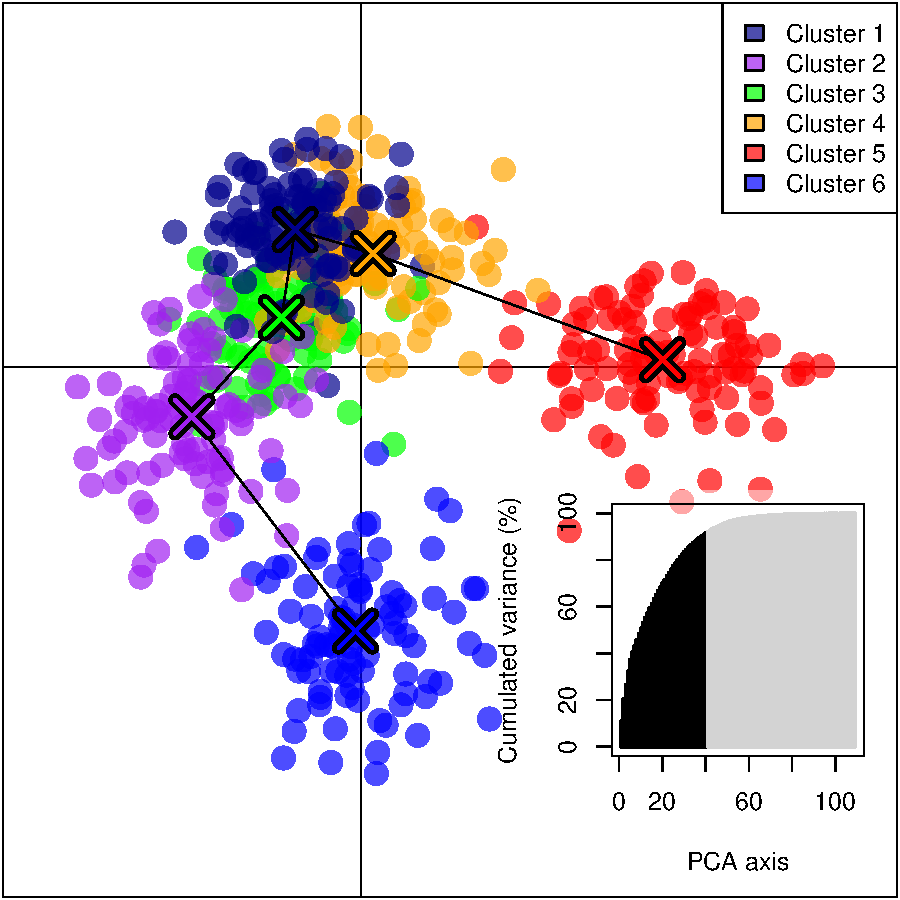
\includegraphics{figs/dapc-014}


Lastly, note that \texttt{scatter} can also represent a single discriminant function, which is
especially useful when only one of these has been retained (e.g. in the case $k=2$).
This is achieved by plotting the densities of individuals on a given discriminant function with
different colors for different groups:
\begin{Schunk}
\begin{Sinput}
> scatter(dapc1, 1, 1, col = myCol, bg = "white", scree.da = FALSE, 
+     legend = TRUE, solid = 0.4)
\end{Sinput}
\end{Schunk}
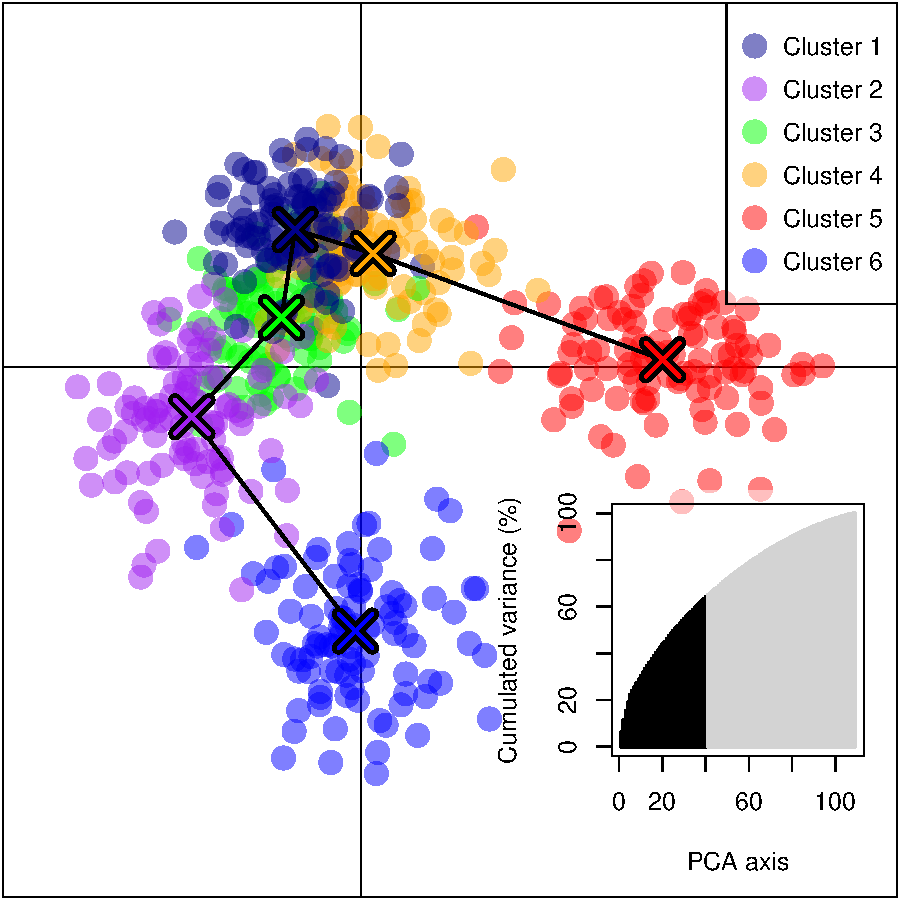
\includegraphics{figs/dapc-015}




%%%%%%%%%%%%%%%%
\subsection{Interpreting variable contributions}
%%%%%%%%%%%%%%%%

In DAPC, the variable actually analyzed are principal components of a PCA.
Loadings of these variables are generally uninformative, since PCs themselves do not all have
straightforward interpretations.
However, we can also compute contributions of the alleles, which can turn out to be very informative.
In general, there are many alleles and their contribution is best plotted for a single discriminant
function at a time.

Variable contributions are stored in the \texttt{var.contr} slot of a \texttt{dapc} object.
They can be plotted using \texttt{loadingplot}.
We illustrate this using the seasonal influenza dataset \texttt{H3N2}, which contains 1903 isolates
genotyped for 125 SNPs located in the hemagglutinin segment (see \texttt{?H3N2}):
\begin{Schunk}
\begin{Sinput}
> data(H3N2)
> H3N2
\end{Sinput}
\begin{Soutput}
   #####################
   ### Genind object ### 
   #####################
- genotypes of individuals - 

S4 class:  genind
@call: .local(x = x, i = i, j = j, drop = drop)

@tab:  1903 x 334 matrix of genotypes

@ind.names: vector of  1903 individual names
@loc.names: vector of  125 locus names
@loc.nall: number of alleles per locus
@loc.fac: locus factor for the  334 columns of @tab
@all.names: list of  125 components yielding allele names for each locus
@ploidy:  1
@type:  codom

Optionnal contents: 
@pop:  - empty -
@pop.names:  - empty -

@other: a list containing: x  xy  epid 
\end{Soutput}
\begin{Sinput}
> pop(H3N2) <- H3N2$other$epid
> dapc.flu <- dapc(H3N2, n.pca = 30, n.da = 10)
\end{Sinput}
\end{Schunk}

The first discriminant function shows the temporal evolution of the influenza virus, while the
second one shows the originality of 2006 strains.
\begin{Schunk}
\begin{Sinput}
> myPal <- colorRampPalette(c("blue", "gold", "red"))
> scatter(dapc.flu, col = transp(myPal(6)), scree.da = FALSE, cell = 1.5, 
+     cex = 2, bg = "white", cstar = 0)
\end{Sinput}
\end{Schunk}
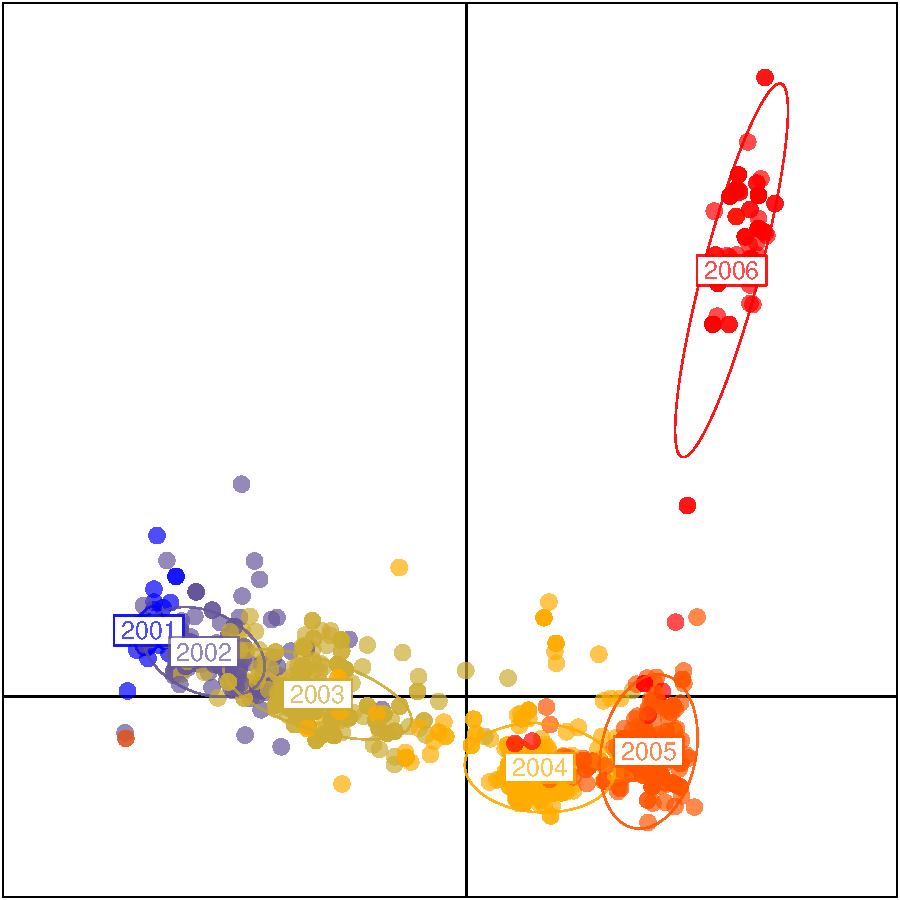
\includegraphics{figs/dapc-017}

We can assess which alleles most highlight the originality of 2006 using \texttt{loadingplot}:
\begin{Schunk}
\begin{Sinput}
> set.seed(4)
> contrib <- loadingplot(dapc.flu$var.contr, axis = 2, thres = 0.07, 
+     lab.jitter = 1)
\end{Sinput}
\end{Schunk}
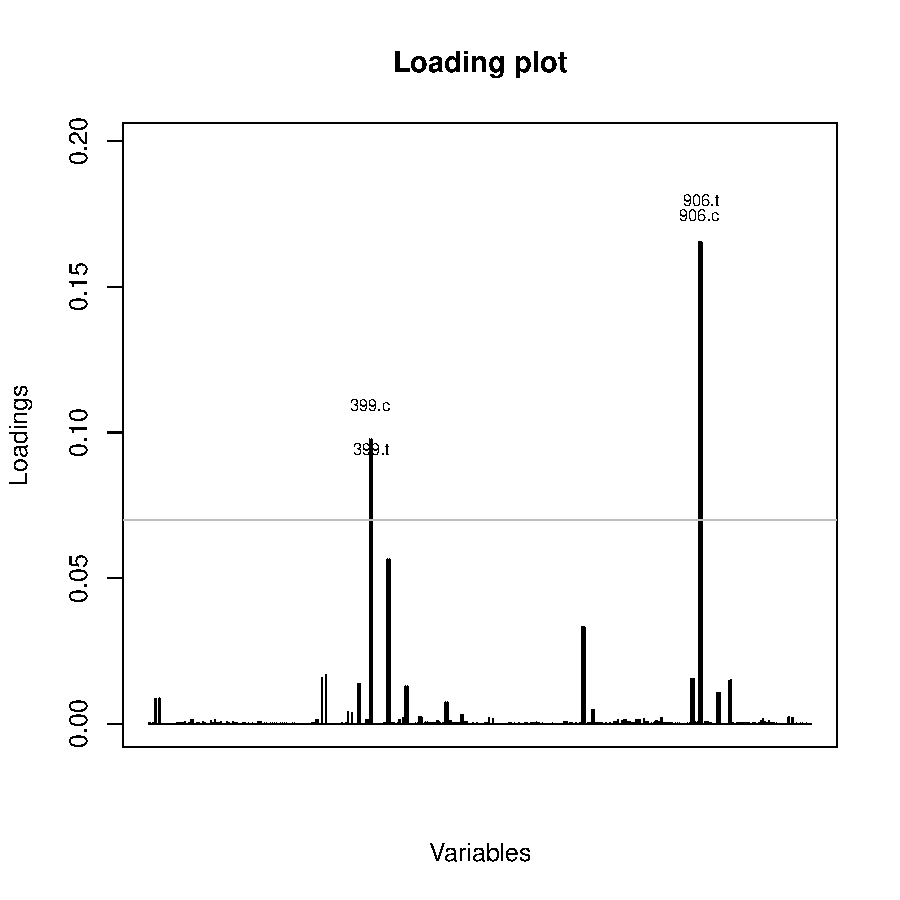
\includegraphics{figs/dapc-018}

\noindent \texttt{temp} is a list invisibly returned by \texttt{loadingplot} which contains the most
contributing alleles (i.e., contributions above a given threshold -- argument \texttt{threshold}).
In this case, SNPs \texttt{906} and \texttt{399} reflect most the temporal evolution of the virus.
We can look into their allele frequencies over 2002-2006:
\begin{Schunk}
\begin{Sinput}
> temp <- seploc(H3N2)
> snp906 <- truenames(temp[["906"]])$tab
> snp399 <- truenames(temp[["399"]])$tab
> freq906 <- apply(snp906, 2, function(e) tapply(e, pop(H3N2), 
+     mean, na.rm = TRUE))
> freq399 <- apply(snp399, 2, function(e) tapply(e, pop(H3N2), 
+     mean, na.rm = TRUE))
> freq906
\end{Sinput}
\begin{Soutput}
           906.c     906.t
2001 0.000000000 1.0000000
2002 0.000000000 1.0000000
2003 0.000000000 1.0000000
2004 0.000000000 1.0000000
2005 0.002155172 0.9978448
2006 0.616071429 0.3839286
\end{Soutput}
\begin{Sinput}
> freq399
\end{Sinput}
\begin{Soutput}
           399.c     399.t
2001 0.000000000 1.0000000
2002 0.000000000 1.0000000
2003 0.000000000 1.0000000
2004 0.001848429 0.9981516
2005 0.002079002 0.9979210
2006 0.357142857 0.6428571
\end{Soutput}
\begin{Sinput}
> par(mfrow = c(1, 2), mar = c(5.1, 4.1, 4.1, 0.1), las = 3)
> matplot(freq906, pch = c("a", "c"), type = "b", xlab = "year", 
+     ylab = "allele frequency", xaxt = "n", cex = 1.5, main = "SNP # 906")
> axis(side = 1, at = 1:6, lab = 2001:2006)
> matplot(freq399, pch = c("c", "t"), type = "b", xlab = "year", 
+     ylab = "allele frequency", xaxt = "n", cex = 1.5, main = "SNP # 399")
> axis(side = 1, at = 1:6, lab = 2001:2006)
\end{Sinput}
\end{Schunk}
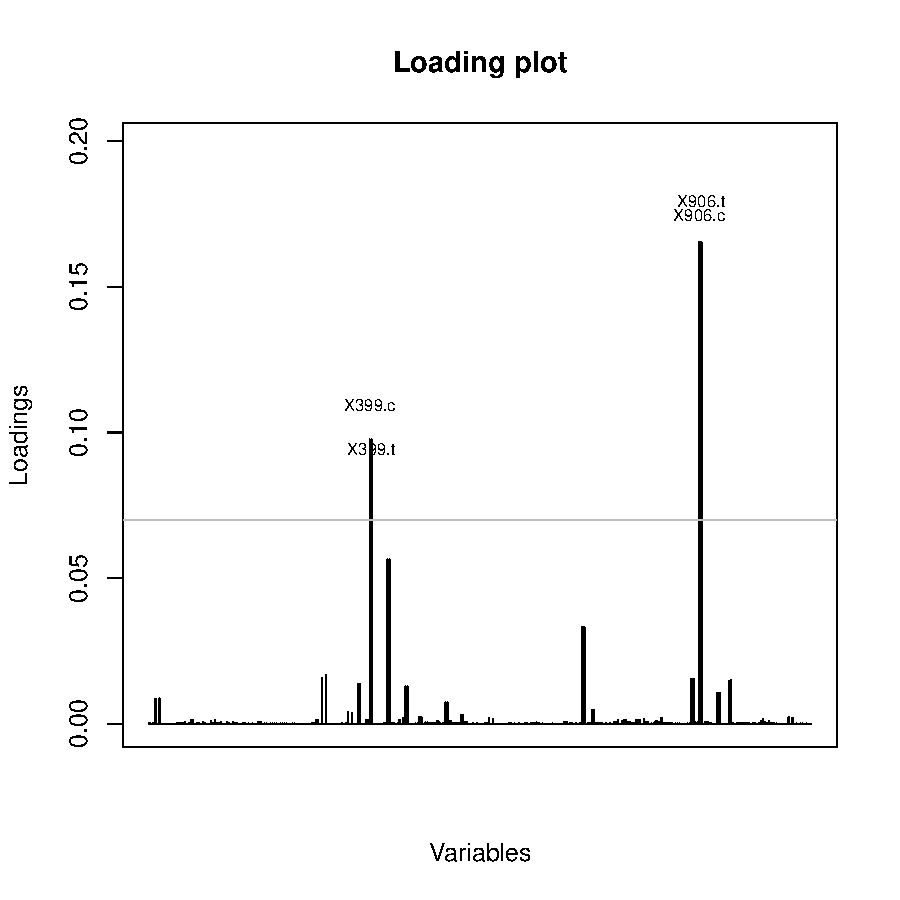
\includegraphics{figs/dapc-019}

In both cases, a new allele appeared in 2005 at a very low frequency, and reached high or even dominant frequencies a
year later.
Irrespective of the mecanism underlying these changes (drift or selection), this illustrates that in
seasonal influenza, specific nucleotides can undergo drastic changes within only a couple of years.




%%%%%%%%%%%%%%%%
\subsection{Interpreting group memberships}
%%%%%%%%%%%%%%%%
Besides scatterplots of discriminant functions, group memberships of DAPC can be exploited.
Note that caution should be taken when interpreting group memberships of a DAPC based on too many
PCs, as there are risks of overfitting the discriminant functions (see section below).
But despite this possible bias, group memberships can be used as indicators of how
clear-cut genetic clusters are.
Note that this is most useful for groups defined by an external criteria, i.e. defined biologically, as opposed to identified by $k$-means.
It is less useful for groups identified using \texttt{find.clusters}, since we expect $k$-means to
provide optimal groups for DAPC, and therefore both classifications to be mostly consistent.
\\

Membership probabilities are based on the retained discriminant functions.
They are stored in \texttt{dapc} objects in the slot \texttt{posterior}:
\begin{Schunk}
\begin{Sinput}
> class(dapc1$posterior)
\end{Sinput}
\begin{Soutput}
[1] "matrix"
\end{Soutput}
\begin{Sinput}
> dim(dapc1$posterior)
\end{Sinput}
\begin{Soutput}
[1] 600   6
\end{Soutput}
\begin{Sinput}
> round(head(dapc1$posterior), 3)
\end{Sinput}
\begin{Soutput}
        1 2 3 4     5 6
001 1.000 0 0 0 0.000 0
002 1.000 0 0 0 0.000 0
003 1.000 0 0 0 0.000 0
004 0.016 0 0 0 0.984 0
005 1.000 0 0 0 0.000 0
006 1.000 0 0 0 0.000 0
\end{Soutput}
\end{Schunk}
Each row corresponds to an individual, each column to a group.
This information can be summarized using \texttt{summary} on the \texttt{dapc} object:
\begin{Schunk}
\begin{Sinput}
> summary(dapc1)
\end{Sinput}
\begin{Soutput}
$n.dim
[1] 5

$n.pop
[1] 6

$assign.prop
[1] 0.9966667

$assign.per.pop
        1         2         3         4         5         6 
1.0000000 1.0000000 0.9901961 1.0000000 0.9904762 1.0000000 

$prior.grp.size

  1   2   3   4   5   6 
 98  97 102  99 105  99 

$post.grp.size

  1   2   3   4   5   6 
 99  97 101  99 105  99 
\end{Soutput}
\end{Schunk}
The slot \texttt{assign.per.pop} indicates the proportions of successful reassignment (based on
the discriminant functions) of individuals to their original clusters. Large values indicate clear-cut
clusters, while low values suggest admixed groups.
\\

This information can also be visualized using \texttt{assignplot} (see \texttt{?assignplot} for display
options); here, we choose to represent only the first 50 individuals to make the figure readable:
\begin{Schunk}
\begin{Sinput}
> assignplot(dapc1, subset = 1:50)
\end{Sinput}
\end{Schunk}
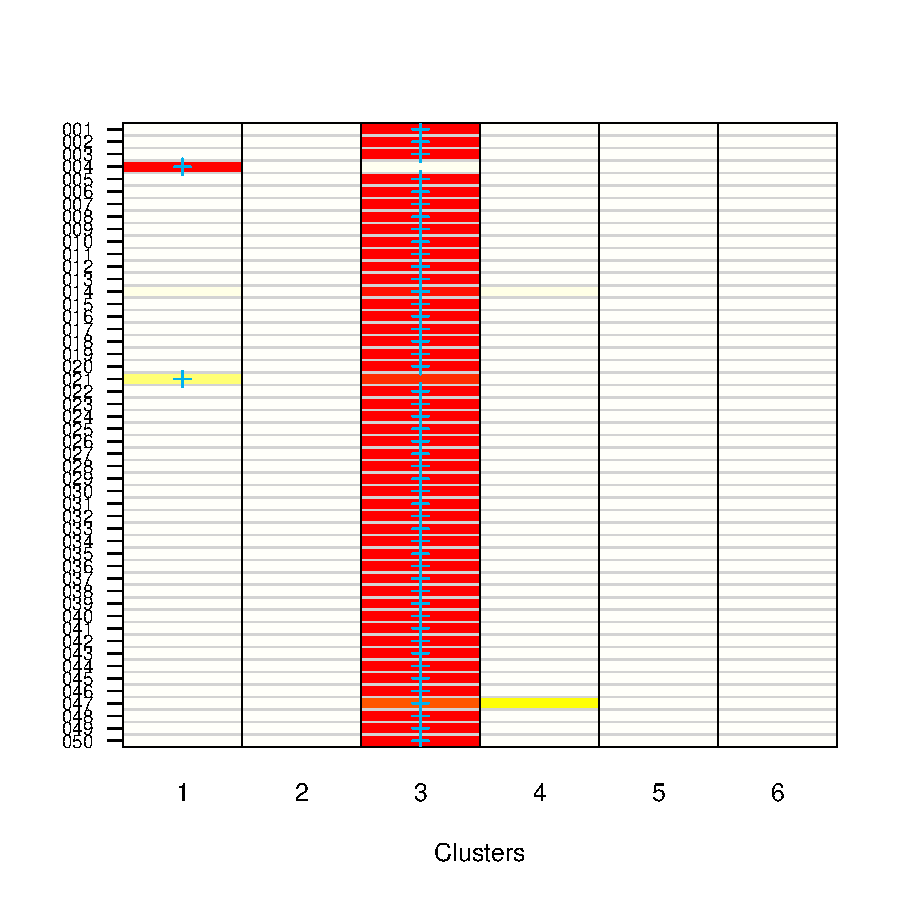
\includegraphics{figs/dapc-022}

\noindent
This figure is the simple graphical translation of the \texttt{posterior} table above. Heat colors
represent membership probabilities
(red=1, white=0); blue crosses represent the prior cluster provided to DAPC.
Here in most individuals, DAPC classification is consistent with the original
clusters (blue crosses are on red rectangles), except for one discrepancy in individual 21, classified
in group 1 while DAPC would assign it to group 3.
Such figure is particularly useful when prior biological groups are used, as one may infer admixed
or misclassified individuals.
\\

Note that this information can also be plotted in a STRUCTURE-like (!) way using \texttt{compoplot}
(see \code{?compoplot} to customize the plot).
We can plot information of all individuals to have a global picture of the clusters composition.
\begin{Schunk}
\begin{Sinput}
> compoplot(dapc1, posi = "bottomright", txt.leg = paste("Cluster", 
+     1:6), lab = "", ncol = 1, xlab = "individuals")
\end{Sinput}
\end{Schunk}
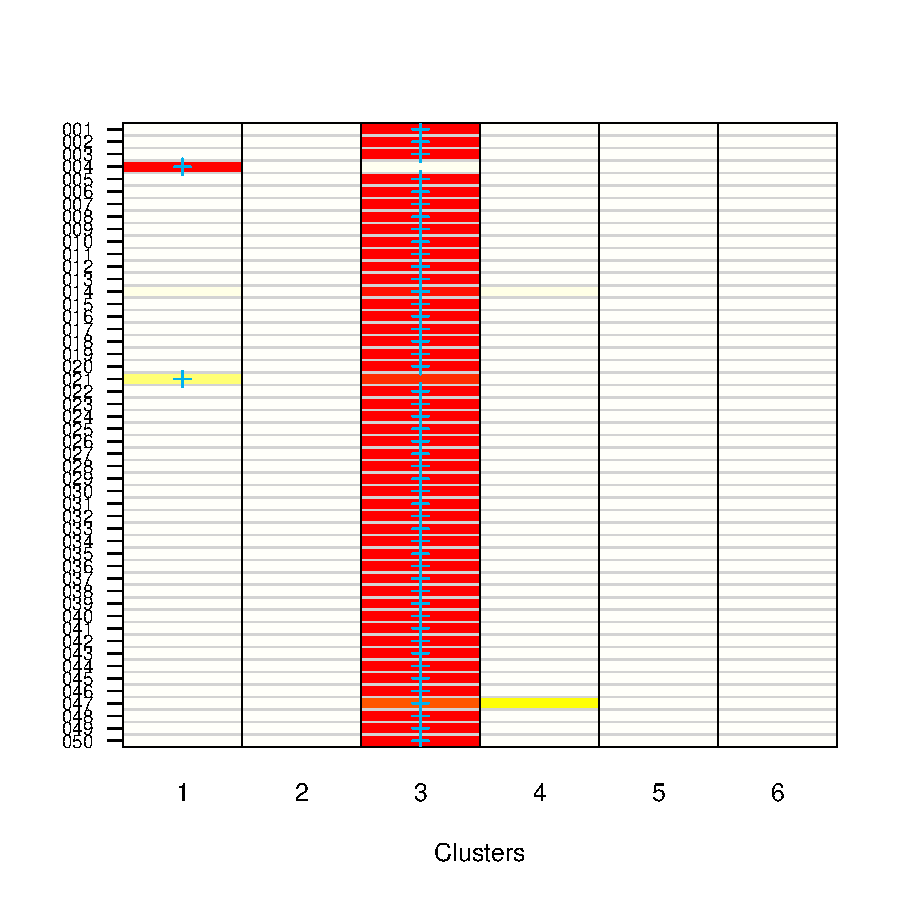
\includegraphics{figs/dapc-023}

\noindent We can also have a closer look at a subset of individuals; for instance, for the first 50 individuals:
\begin{Schunk}
\begin{Sinput}
> compoplot(dapc1, subset = 1:50, posi = "bottomright", txt.leg = paste("Cluster", 
+     1:6), lab = "", ncol = 2, xlab = "individuals")
\end{Sinput}
\end{Schunk}
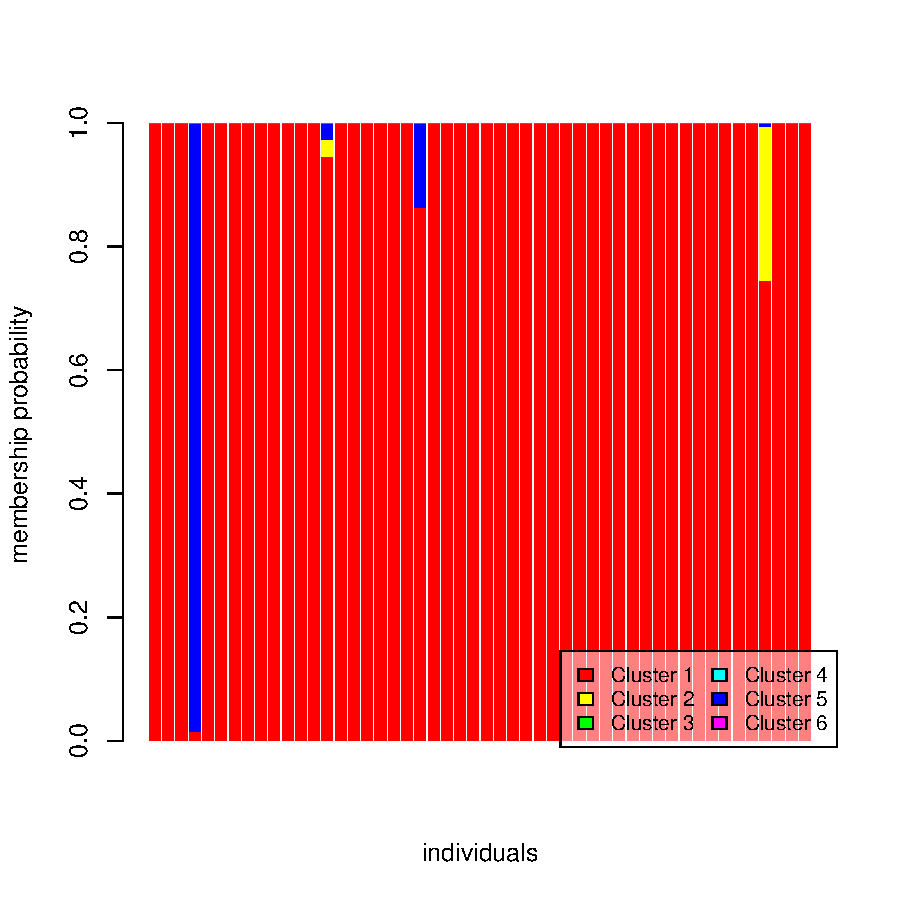
\includegraphics{figs/dapc-024}

Obviously, we can use the power of R to lead our investigation further. For instance, which are the
most 'admixed' individuals?
Let us consider as admixed individuals having no more than 90\% of probability of membership in a single cluster:
\begin{Schunk}
\begin{Sinput}
> temp <- which(apply(dapc1$posterior, 1, function(e) all(e < 0.9)))
> temp
\end{Sinput}
\begin{Soutput}
021 047 243 280 
 21  47 243 280 
\end{Soutput}
\begin{Sinput}
> compoplot(dapc1, subset = temp, posi = "bottomright", txt.leg = paste("Cluster", 
+     1:6), ncol = 2)
\end{Sinput}
\end{Schunk}
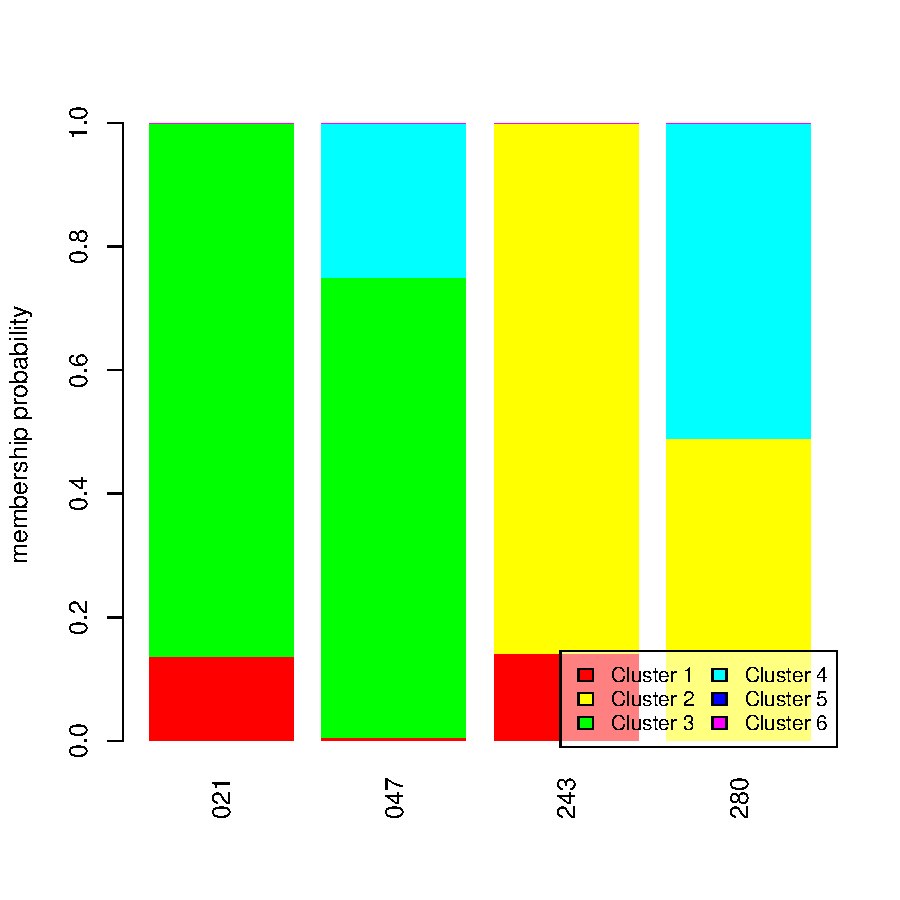
\includegraphics{figs/dapc-025}





%%%%%%%%%%%%%%%%
%%%%%%%%%%%%%%%%
\section{On the stability of group membership probabilities}
%%%%%%%%%%%%%%%%
%%%%%%%%%%%%%%%%


%%%%%%%%%%%%%%%%
\subsection{When and why group memberships can be unreliable}
%%%%%%%%%%%%%%%%

In DAPC, discriminant functions are linear combinations of variables (principal components of PCA) which
optimize the separation of individuals into pre-defined groups. Based on the retained discriminant
functions, it is possible to derive group membership probabilities, which can be interpreted in
order to assess how clear-cut or admixed the clusters are.
Unfortunately, retaining too many PCs with respect to the number of individuals can lead to over-fitting the discriminant functions.
In such case, discriminant functions become so "flexible" that they could discriminate almost perfectly any cluster.
As a result, membership probabilities can become drastically inflated for the best-fitting cluster, resulting in apparent perfect discrimination.
\\


This point can be illustrated using the \texttt{microbov} dataset (704 cattles of 15 breeds typed
for 30 microsatellite markers).
We first examine the  \% of successful reassignment (i.e., quality of discrimination) for different numbers of retained PCs.
First, retaining 3 PCs during the dimension-reduction step, and all discriminant functions:
\begin{Schunk}
\begin{Sinput}
> data(microbov)
> microbov
\end{Sinput}
\begin{Soutput}
   #####################
   ### Genind object ### 
   #####################
- genotypes of individuals - 

S4 class:  genind
@call: genind(tab = truenames(microbov)$tab, pop = truenames(microbov)$pop)

@tab:  704 x 373 matrix of genotypes

@ind.names: vector of  704 individual names
@loc.names: vector of  30 locus names
@loc.nall: number of alleles per locus
@loc.fac: locus factor for the  373 columns of @tab
@all.names: list of  30 components yielding allele names for each locus
@ploidy:  2
@type:  codom

Optionnal contents: 
@pop:  factor giving the population of each individual
@pop.names:  factor giving the population of each individual

@other: a list containing: coun  breed  spe 
\end{Soutput}
\begin{Sinput}
> temp <- summary(dapc(microbov, n.da = 100, n.pca = 3))$assign.per.pop * 
+     100
\end{Sinput}
\end{Schunk}
\begin{Schunk}
\begin{Sinput}
> par(mar = c(4.5, 7.5, 1, 1))
> barplot(temp, xlab = "% of reassignment to actual breed", horiz = TRUE, 
+     las = 1)
\end{Sinput}
\end{Schunk}
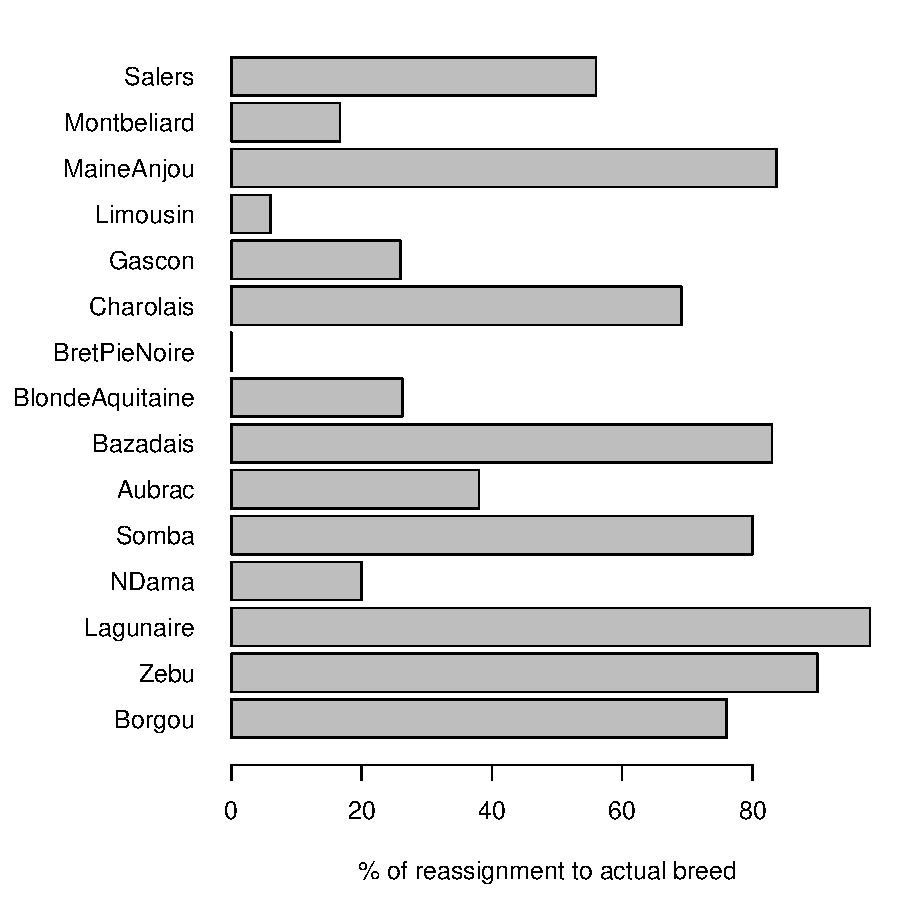
\includegraphics{figs/dapc-027}

\noindent
We can see that some breeds are well discriminated (e.g. Zebu, Lagunaire,  > 90\%) while others are
entirely overlooked by the analysis (e.g. Bretone Pie Noire, Limousin, <10\%).
This is because too much genetic information is lost when retaining only 3 PCs.
We repeat the analysis, this time keeping 300 PCs:
\begin{Schunk}
\begin{Sinput}
> temp <- summary(dapc(microbov, n.da = 100, n.pca = 300))$assign.per.pop * 
+     100
\end{Sinput}
\end{Schunk}
\begin{Schunk}
\begin{Sinput}
> par(mar = c(4.5, 7.5, 1, 1))
> barplot(temp, xlab = "% of reassignment to actual breed", horiz = TRUE, 
+     las = 1)
\end{Sinput}
\end{Schunk}
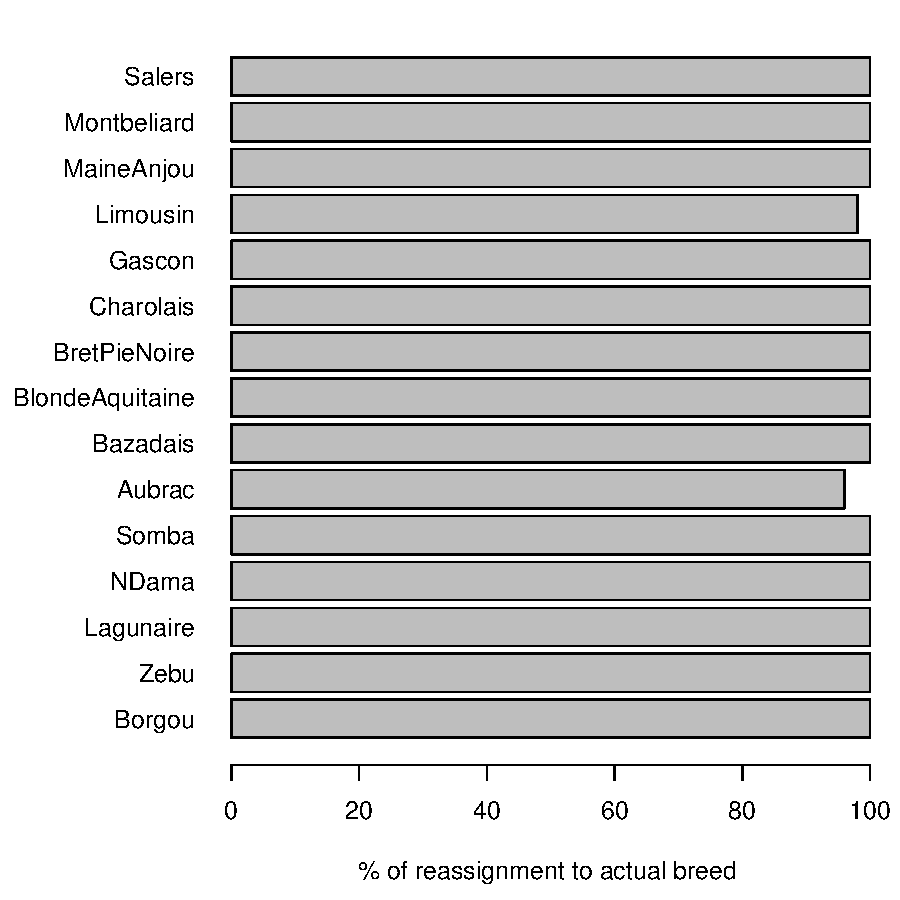
\includegraphics{figs/dapc-029}

\noindent We now obtain almost 100\% of discrimination for all groups.
Is this result satisfying? Actually not.
The number of PCs retained is so large that discriminant functions could model any structure and
virtually any set of clusters would be well discriminated.
This can be illustrated by running the analysis using randomized groups:
\begin{Schunk}
\begin{Sinput}
> x <- microbov
> pop(x) <- sample(pop(x))
> temp <- summary(dapc(x, n.da = 100, n.pca = 300))$assign.per.pop * 
+     100
\end{Sinput}
\end{Schunk}
\begin{Schunk}
\begin{Sinput}
> par(mar = c(4.5, 7.5, 1, 1))
> barplot(temp, xlab = "% of reassignment to actual breed", horiz = TRUE, 
+     las = 1)
\end{Sinput}
\end{Schunk}
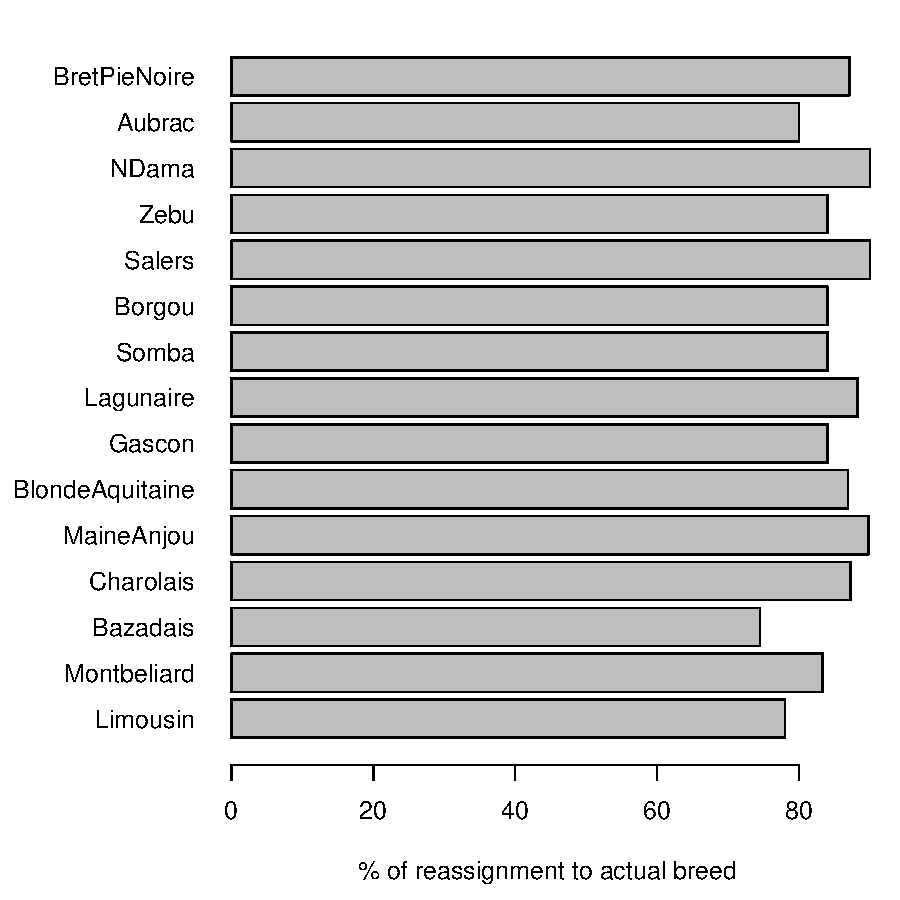
\includegraphics{figs/dapc-031}

\noindent
Groups have been randomised, and yet we still get very good discrimination.
There is therefore a trade-off between finding a space with a good power of discrimination using
DAPC, and retaining too many dimensions and cause over-fitting.




%%%%%%%%%%%%%%%%
\subsection{Using the $a$-score}
%%%%%%%%%%%%%%%%
The trade-off between power of discrimination and over-fitting can be measured by the $a$-score, which is simply the difference between the proportion of
successful reassignment of the analysis (observed discrimination) and values obtained using random
groups (random discrimination).
It can be seen as the proportion of successful reassignment corrected for the number of retained PCs.
It is implemented by \texttt{a.score}, which relies on repeating the DAPC analysis using randomized
groups, and computing $a$-scores for each group, as well as the average $a$-score:
\begin{Schunk}
\begin{Sinput}
> dapc2 <- dapc(microbov, n.da = 100, n.pca = 10)
> temp <- a.score(dapc2)
> names(temp)
\end{Sinput}
\begin{Soutput}
[1] "tab"       "pop.score" "mean"     
\end{Soutput}
\begin{Sinput}
> temp$tab[1:5, 1:5]
\end{Sinput}
\begin{Soutput}
      Borgou Zebu Lagunaire     NDama Somba
sim.1   0.74 0.84 0.8235294 0.5666667  0.58
sim.2   0.76 0.72 0.8627451 0.5333333  0.78
sim.3   0.60 0.78 0.8627451 0.5000000  0.70
sim.4   0.64 0.74 0.8627451 0.5333333  0.70
sim.5   0.72 0.76 0.9607843 0.5000000  0.80
\end{Soutput}
\begin{Sinput}
> temp$pop.score
\end{Sinput}
\begin{Soutput}
         Borgou            Zebu       Lagunaire           NDama           Somba 
      0.6380000       0.7420000       0.8509804       0.5166667       0.7180000 
         Aubrac        Bazadais BlondeAquitaine    BretPieNoire       Charolais 
      0.4940000       0.8382979       0.3016393       0.4741935       0.5563636 
         Gascon        Limousin      MaineAnjou     Montbeliard          Salers 
      0.6640000       0.4280000       0.8653061       0.6733333       0.7720000 
\end{Soutput}
\begin{Sinput}
> temp$mean
\end{Sinput}
\begin{Soutput}
[1] 0.6355187
\end{Soutput}
\end{Schunk}

The number of retained PCs can be chosen so as to optimize the $a$-score; this is achived by \texttt{optim.a.score}:
\begin{Schunk}
\begin{Sinput}
> dapc2 <- dapc(microbov, n.da = 100, n.pca = 50)
\end{Sinput}
\end{Schunk}
\begin{Schunk}
\begin{Sinput}
> temp <- optim.a.score(dapc2)
\end{Sinput}
\end{Schunk}
\begin{center}
  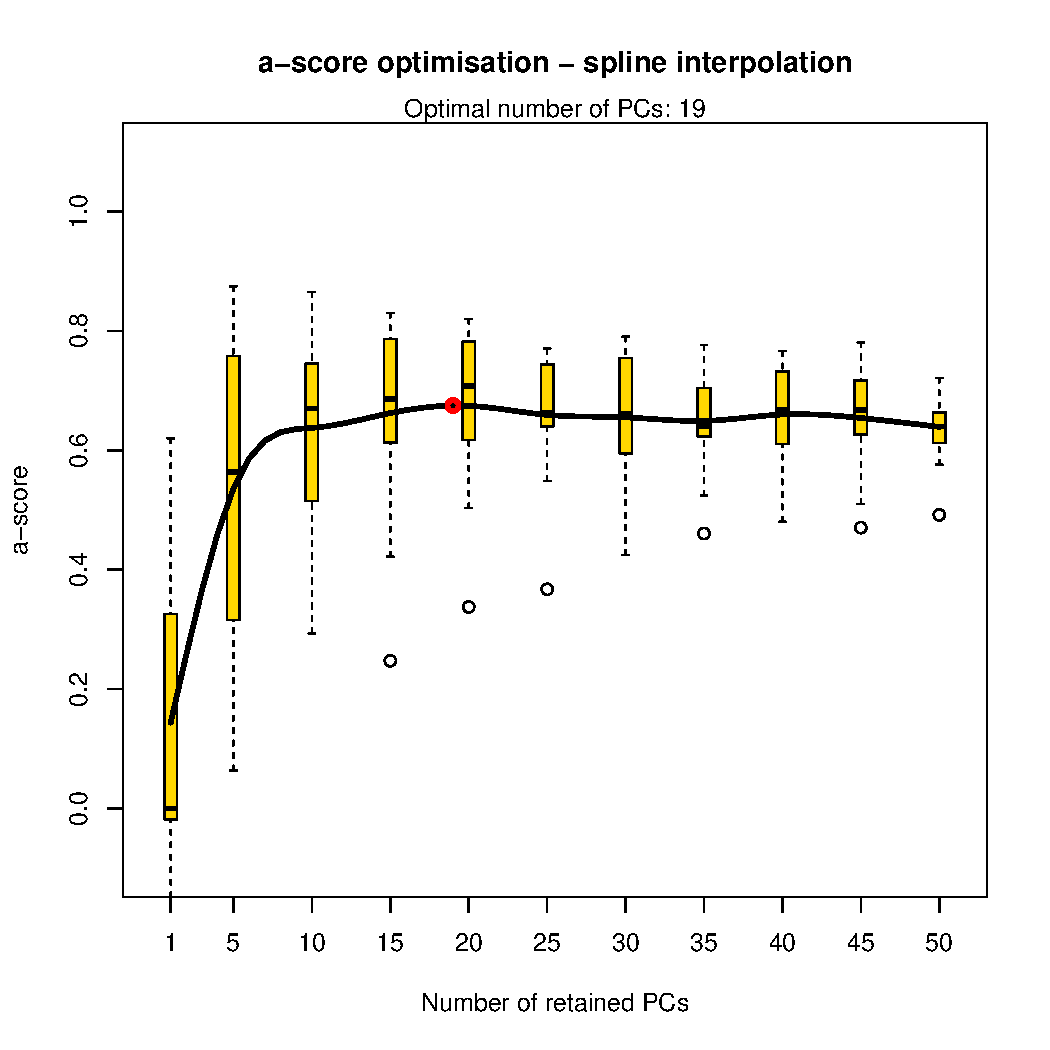
\includegraphics[width=.7\textwidth]{figs/ascore.pdf}
\end{center}


\noindent Since evaluating solutions for 1, 2, ... 100 retained PCs is unusefully computer-intensive, as a first approximation the
method evaluates a few numbers of retained PCs in this range, and uses spline interpolation to
approximate the optimal number of PCs to retain. Then, one can evaluate all solutions within a
restrained range using the argument \texttt{n.pca}.
For the \texttt{microbov} dataset, we should probably retained between 10 and 30 PCs during the
dimension-reduction step.
\\

We perform the analysis with 20 PCs retained, and then map the membership probabilities as before:
\begin{Schunk}
\begin{Sinput}
> dapc3 <- dapc(microbov, n.da = 100, n.pca = 20)
> myCol <- rainbow(15)
\end{Sinput}
\end{Schunk}
\begin{Schunk}
\begin{Sinput}
> par(mar = c(5.1, 4.1, 1.1, 1.1), xpd = TRUE)
> compoplot(dapc3, lab = "", posi = list(x = 12, y = -0.01), cleg = 0.7)
\end{Sinput}
\end{Schunk}
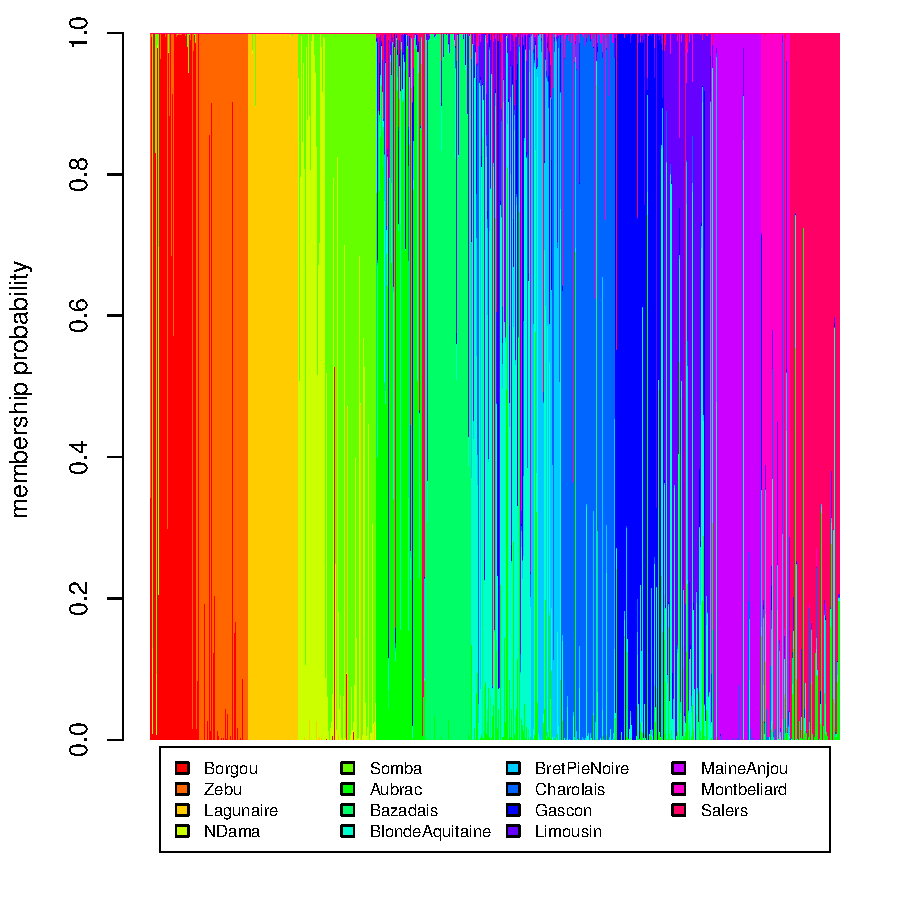
\includegraphics{figs/dapc-036}

And as before, we can investigate further admixed individuals, which we arbitrarily define as those
having no more than 0.5 probability of membership to any group:
\begin{Schunk}
\begin{Sinput}
> temp <- which(apply(dapc3$posterior, 1, function(e) all(e < 0.5)))
> temp
\end{Sinput}
\begin{Soutput}
 AFBIBOR9511  FRBTAUB9062  FRBTAUB9070  FRBTAUB9078  FRBTAUB9225 FRBTBDA29851 
           9          233          241          249          265          329 
FRBTBDA29856 FRBTBDA29879 FRBTBDA35248 FRBTBDA35256 FRBTBDA35259 FRBTBDA35267 
         334          354          361          363          365          368 
FRBTBDA35278 FRBTBDA35281 FRBTBDA35877 FRBTBDA35941  FRBTBPN1906  FRBTBPN1913 
         372          374          382          386          405          409 
 FRBTBPN1915 FRBTCHA15957 FRBTGAS14183  FRBTGAS9173  FRBTGAS9200 FRBTLIM30832 
         411          422          477          498          520          543 
FRBTLIM30839 FRBTLIM30855  FRBTMA25298  FRBTMBE1496  FRBTMBE1514  FRBTMBE1544 
         550          566          579          625          636          651 
\end{Soutput}
\begin{Sinput}
> lab <- pop(microbov)
> par(mar = c(8, 4, 5, 1), xpd = TRUE)
> compoplot(dapc3, subset = temp, cleg = 0.6, posi = list(x = 0, 
+     y = 1.2), lab = lab)
\end{Sinput}
\end{Schunk}
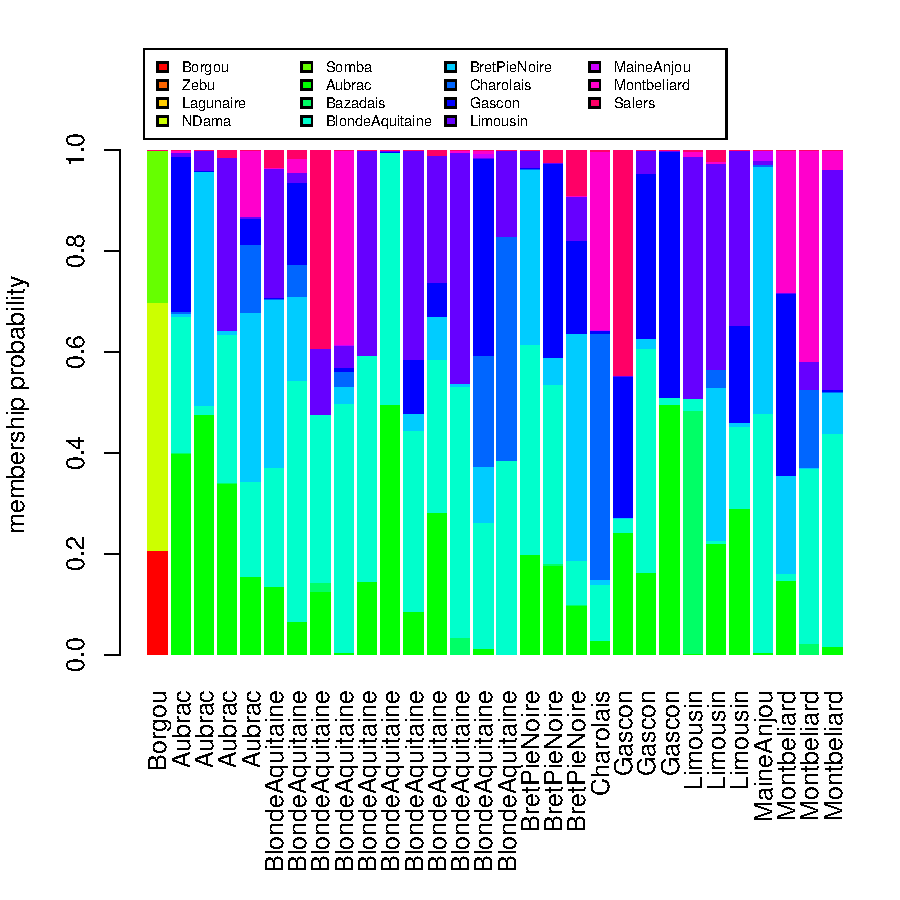
\includegraphics{figs/dapc-037}

\noindent Admixture appears to be the strongest between a few breeds (Blonde d'Aquitaine, Bretonne Pie-Noire,
Limousine and Gascone). Some features are fairly surprising; for instance, the last individual is
fairly distant from its cluster, but has almost 50\% chances of being assigned to two other breeds.






%%%%%%%%%%%%%%%%
%%%%%%%%%%%%%%%%
\section{Using supplementary individuals}
%%%%%%%%%%%%%%%%
%%%%%%%%%%%%%%%%

%%%%%%%%%%%%%%%%
\subsection{Rationale}
%%%%%%%%%%%%%%%%

Statistically speaking, supplementary individuals are observations which do not participate to
constructing a model, but which we would like to predict using a model fitted on other ("training") data.
In the context of DAPC, we may know groups for most individuals, but some individuals could be of
unknown or uncertain group. In this case, we need to exclude individuals from the analysis, and then
project them as supplementary individuals onto the discriminant functions.
The only requirement for this operation is that supplementary individuals have been typed for the
same loci as the rest of the dataset.

Technically, using supplementary individuals consists in transforming the new data using the centring
and scaling of the "training data", and then using the same discriminant coefficients as
for the contributing individuals to predict the position of the new individuals onto the
discriminant functions.


%%%%%%%%%%%%%%%%
\subsection{In practice}
%%%%%%%%%%%%%%%%
We will illustrate the practice of supplementary individuals using the cattle breeds data previously
analyzed (\texttt{microbov} dataset).
We first split the dataset into two parts: one used for the analysis, and one used as supplementary individuals:
\begin{Schunk}
\begin{Sinput}
> data(microbov)
> set.seed(2)
> kept.id <- unlist(tapply(1:nInd(microbov), pop(microbov), function(e) sample(e, 
+     20, replace = FALSE)))
> x <- microbov[kept.id]
> x.sup <- microbov[-kept.id]
> nInd(x)
\end{Sinput}
\begin{Soutput}
[1] 300
\end{Soutput}
\begin{Sinput}
> nInd(x.sup)
\end{Sinput}
\begin{Soutput}
[1] 404
\end{Soutput}
\end{Schunk}
\texttt{x} is a \texttt{genind} containing the data to be analyzed; \texttt{x.sup} contains the
supplementary individuals.


We perform the DAPC of \texttt{x}, and use \texttt{predict} to predict results for the
supplementary individuals:
\begin{Schunk}
\begin{Sinput}
> dapc4 <- dapc(x, n.pca = 20, n.da = 15)
> pred.sup <- predict.dapc(dapc4, newdata = x.sup)
> names(pred.sup)
\end{Sinput}
\begin{Soutput}
[1] "assign"     "posterior"  "ind.scores"
\end{Soutput}
\begin{Sinput}
> head(pred.sup$assign)
\end{Sinput}
\begin{Soutput}
[1] Borgou Borgou Borgou Borgou Borgou Borgou
15 Levels: Borgou Zebu Lagunaire NDama Somba Aubrac ... Salers
\end{Soutput}
\begin{Sinput}
> pred.sup$ind.scores[1:5, 1:3]
\end{Sinput}
\begin{Soutput}
          LD1       LD2        LD3
001 -3.896992 -5.288381  0.4570651
002 -2.445063 -4.422078  0.2134797
003 -4.692576 -2.717198  0.4914203
004 -4.919515 -2.317070 -0.2390356
005 -4.718570 -0.200391 -0.9196541
\end{Soutput}
\begin{Sinput}
> round(pred.sup$posterior[1:5, 1:5], 3)
\end{Sinput}
\begin{Soutput}
    Borgou  Zebu Lagunaire NDama Somba
001  0.612 0.388         0 0.000 0.000
002  0.983 0.017         0 0.000 0.000
003  1.000 0.000         0 0.000 0.000
004  1.000 0.000         0 0.000 0.000
005  0.688 0.000         0 0.208 0.105
\end{Soutput}
\end{Schunk}

\noindent The list \texttt{pred.sup} contains all the predictions about the new data based on the
analysis stored in \texttt{dapc4}. The slot \texttt{assign} contains the assignment of new individuals
to groups; \texttt{ind.scores} contains the coordinates of the new individuals on the discriminant
functions; \texttt{posterior} contains the posterior membership probabilities.
We can visualize the information by different ways.
First, we can represent the new individuals using a scatterplot:
\begin{Schunk}
\begin{Sinput}
> col <- rainbow(length(levels(pop(x))))
> col.points <- transp(col[as.integer(pop(x))], 0.2)
> scatter(dapc4, col = col, bg = "white", scree.da = 0, pch = "", 
+     cstar = 0, clab = 0, xlim = c(-10, 10), legend = TRUE)
> par(xpd = TRUE)
> points(dapc4$ind.coord[, 1], dapc4$ind.coord[, 2], pch = 20, 
+     col = col.points, cex = 5)
> col.sup <- col[as.integer(pop(x.sup))]
> points(pred.sup$ind.scores[, 1], pred.sup$ind.scores[, 2], pch = 15, 
+     col = transp(col.sup, 0.7), cex = 2)
> add.scatter.eig(dapc4$eig, 15, 1, 2, posi = "bottomright", inset = 0.02)
\end{Sinput}
\end{Schunk}
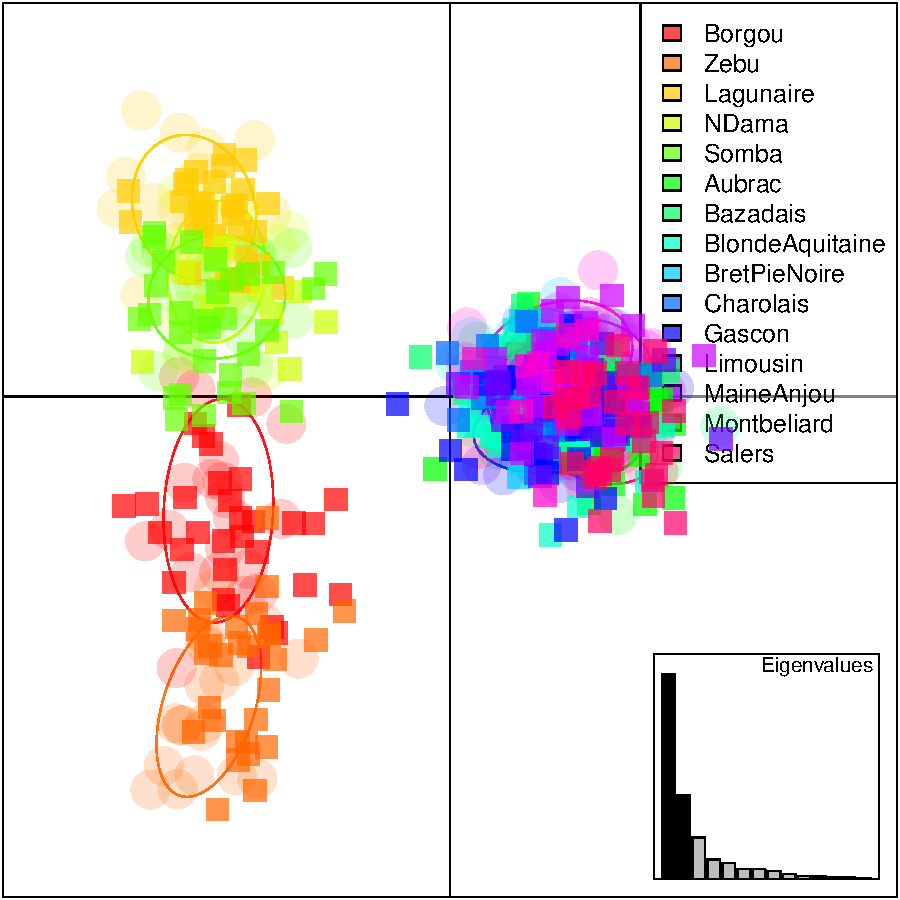
\includegraphics{figs/dapc-040}

\noindent Light dots and ellipses correspond to the original analysis, while more solid squares indicate
supplementary individuals.
Results are fairly satisfying:
\begin{Schunk}
\begin{Sinput}
> mean(as.character(pred.sup$assign) == as.character(pop(x.sup)))
\end{Sinput}
\begin{Soutput}
[1] 0.7549505
\end{Soutput}
\end{Schunk}
Around 75\% of
individuals have been assigned to their actual cluster.
For more details about which breed was assigned to which cluster, we can display the contingency
table of the actual cluster \textit{vs} the inferred one:
\begin{Schunk}
\begin{Sinput}
> table.value(table(pred.sup$assign, pop(x.sup)), col.lab = levels(pop(x.sup)))
\end{Sinput}
\end{Schunk}
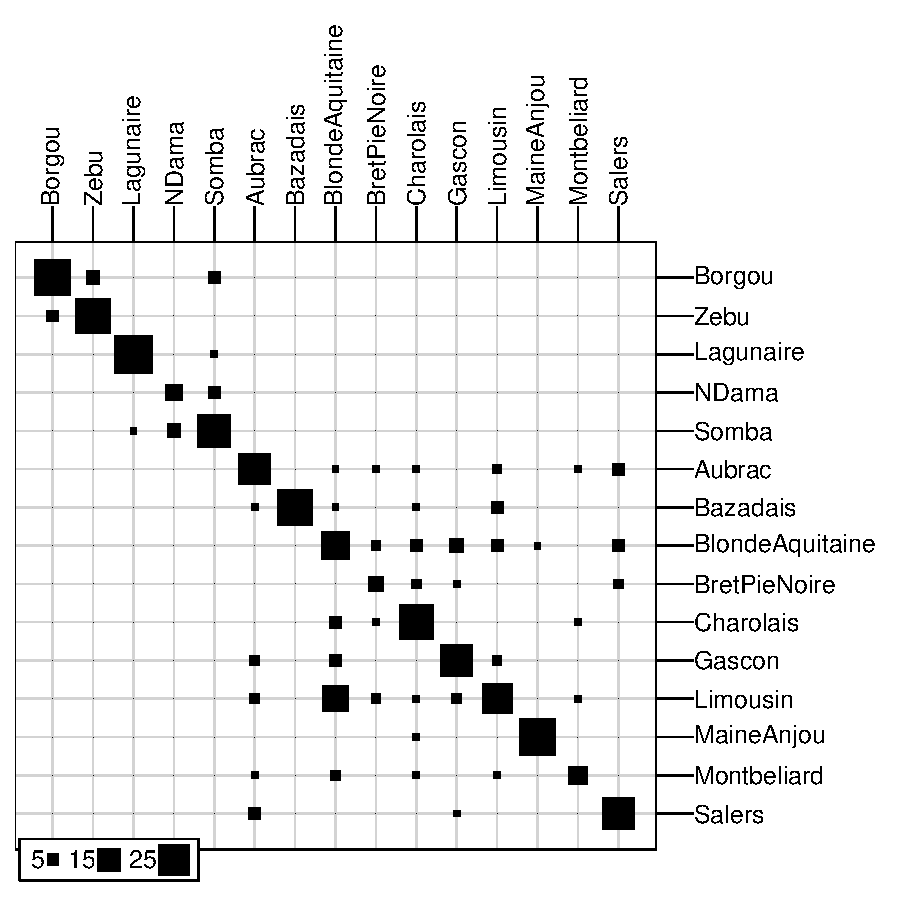
\includegraphics{figs/dapc-042}

\noindent Columns correspond to actual clusters of the supplementary individuals, while rows
correspond to inferred clusters.
Overall, groups are fairly well retrieved, but we can notice that individuals of Blonde d'Aquitaine
breed are poorly identified compared to other breeds.

\begin{thebibliography}{9}

\bibitem{tjart19}
  Jombart T, Devillard S and Balloux, F (2010).
  Discriminant analysis of principal components: a new method for the analysis of genetically structured populations.
  \textit{BMC Genetics} 11: 94.

\bibitem{tjart05}
  Jombart, T. (2008) adegenet: a R package for the multivariate
  analysis of genetic markers. \textit{Bioinformatics} 24: 1403-1405.

\bibitem{np145}
  R Development Core Team (2011). R: A language and environment for
  statistical computing. R Foundation for Statistical Computing,
  Vienna, Austria. ISBN 3-900051-07-0.

\end{thebibliography}

\end{document}
